\documentclass{uvamscse}

\usepackage{listings}

\lstdefinelanguage{sdf}{%
  numbers=none,
  morekeywords={module,imports,exports,sorts,context,lexical,free,syntax,==,=,+,-,left,cons,prefer,avoid,bracket},
  columns=flexible,
  morestring=[b]",
  basicstyle=\footnotesize\mdseries,
  literate={->}{{\,\,$\to$\,\,}}1
}

\lstdefinelanguage{dcg}{%
  numbers=none,
  morekeywords={},
  morestring=[b]",
  basicstyle=\footnotesize\mdseries,
  columns=flexible,
}

\lstdefinelanguage{prolog},
  literate={:-}{{\,$\Leftarrow$\,\,}}1 {-->}{{$\to$\,}}1
}

\lstdefinestyle{mono}{
  basicstyle=\footnotesize\ttfamily
}

\lstdefinelanguage{scala}{
  morekeywords={abstract,case,catch,class,def,%
    do,else,extends,false,final,finally,%
    for,if,implicit,import,match,mixin,%
    new,null,object,override,package,%
    private,protected,requires,return,sealed,%
    super,this,throw,trait,true,try,%
    type,val,var,while,with,yield},
  otherkeywords={=>,<-,<\%,<:,>:,\#,@},
  sensitive=true,
  morecomment=[l]{//},
  morecomment=[n]{/*}{*/},
  morestring=[b]",
  morestring=[b]',
  morestring=[b]"""
}

\lstset{%
  frame=none,
  xleftmargin=2pt,
  stepnumber=1,
  numbers=left,
  numbersep=7pt,
  numberstyle=\ttfamily\scriptsize\color[gray]{0.3},
  belowcaptionskip=\bigskipamount,
  captionpos=b,
%  escapeinside={*'}{'*},
  % language=fl,
  tabsize=2,
  emphstyle={\bf},
  stringstyle=\itshape,
  showspaces=false,
  keywordstyle=\bfseries\rmfamily,
  columns=flexible,
  basicstyle=\small\mdseries,
  showstringspaces=false,
}

\newcommand{\cmd}[1]{\texttt{$\backslash$#1}}

\title{Automated testing}
\subtitle{A Thesis Template Leading by Example}
% \date{Spring 2014}

\author{Thanusijan Tharumarajah}
\authemail{tthanusijan@gmail.com}
\host{ING Bank, The Netherlands, \url{www.ing.nl}}

\supervisor{Prof.dr J.J. Vinju}

%%%%%%%%%%%%%%%%%%%%%%%%%%%%%%%%%%%%%%%%%%%%%%%%%%%%%%%%%%%%%%%%%%%%%%%%%%%%%%%

% Abstract
\abstract{
  This section summarises the content of the thesis for potential readers who do not have time to read it whole,
  or for those undecided whether to read it at all. Sum up the following aspects:

  \begin{itemize}
    \item relevance and motivation for the research
    \item research question(s) and a brief description of the research method
    \item results, contributions and conclusions
  \end{itemize}
}

%%%%%%%%%%%%%%%%%%%%%%%%%%%%%%%%%%%%%%%%%%%%%%%%%%%%%%%%%%%%%%%%%%%%%%%%%%%%%%%

\begin{document}
\maketitle

\listoftodos[Todo's]

% Chapters

%%%%%%%%%%%%%%%%%%%%%%%%%%%%%%%%%%%%%%%%%%%%%%%%%%%%%%%%%%%%%%%%%%%%%%%%%%%%%%%

% Introduction
\chapter{Introduction}

\epigraph{Discovering the unexpected is more important than confirming the
known.}{George E. P. Box}

Growing systems is a concern for large
organisations.~\cite[p.~1]{stoel_storm_vinju_bosman_2016} The continuity of
systems becomes difficult and a single modification can result in unexpected
behaviour of a larger part of the system.

Within the domain knowledge, reasoning about the expected behaviour of a system,
changes and errors are hard. \textit{Rebel} aims to solve these challenges by centralising the domain knowledge and relating
it to the running systems. \textit{Rebel} is a formal specification language which is
used for controlling the intrinsic complexity of software for financial
enterprise systems.~\cite[p.~1]{stoel_storm_vinju_bosman_2016}

Software testing is an important part in software projects.~\cite[p.~4]{myers2011art} The testing
process within large systems can be challenging, it entails not only defining
and executing a lot of test cases, solving thousands of errors, handling
thousands of modules, but also enormous project management. To facilitate this
process \textit{Rebel} offers automated simulation and checking of specifications with
the use of a Satisfiability Modulo Theories (SMT) solver. This solves to some
extent the testing and reasoning of \textit{Rebel} specifications, but this is only
within in the \textit{Rebel} domain.

With the use of code generators, code can be
generated from \textit{Rebel} specifications. The problem with code generation is that the resulting
product is leaving the \textit{Rebel} domain, causing loss of testing and reasoning with
the use of formal methods. The challenge is to regain the benefits from the
\textit{Rebel} domain to be able to test and reason about running systems.
% The challenge is to regain the benefits from the \textit{Rebel} domain to be able to test and reason about systems with the use of formal methods.

\section{Problem statement}\label{sec:problem-statement}

% Ultimately, running systems should be generated from \textit{Rebel} specifications. Since \textit{Rebel} is a declarative language it will not always be straightforward to generate a correct system from this. Again SMT solvers might hold the key as shown in other work like [9].

According to the study~\cite[p.~3]{stoelcase} it should be possible to generate
running systems from \textit{Rebel} specifications. Right now this is possible and
running systems are generated from \textit{Rebel} specifications. It isn't always straightforward to generate a correct system from \textit{Rebel}
specifications since \textit{Rebel} is a declarative language.~\cite[p.~3]{stoelcase}
As mentioned before, the simulation and checking for the correctness of
specifications is only in the \textit{Rebel} domain.

The running systems which are
generated from specifications need to be properly based on these specifications,
it should be conform to these specifications. So additional work is necessary for
the generation process to know that running systems are conform to the
specifications.

The language \textit{Rebel} promised to be deterministic, this also holds
for the generated system. So nondeterministic behaviour should be identified.

For ING Bank it is especially important that there is no corrupted data within
the runtime systems.

\subsection{Research questions}\label{sec:research-questions}
The following questions are defined to achieve the research goal:

\begin{description}
  \item [RQ] How to validate the generated code from a Rebel specification?

  \begin{description}
    \item [SQ1] How is the input/output of the generated system tested?
    \item [SQ2] Are there any false positives/negatives when the generated
    system has been implemented correctly?
    \item [SQ3] What kind of bugs can be found and what are the factors?
  \end{description}

\end{description}

\subsection{Research method}\label{sec:research-method}

The research is about testing the implementation correctness of specifications.
For the problems in \autoref{sec:problem-statement}, the
study~\cite[p.3]{stoelcase} proposed a possible solution for these problems,
which is to use SMT Solvers. As before mentioned, the mapping of the \textit{Rebel}
language to the SMT formulas makes it possible to check and simulate
specifications. Hereby, there is an interpreter for \textit{Rebel} specifications, which
is the SMT Solver.~\cite[p.5]{stoel_storm_vinju_bosman_2016}

In the same study,
an attempt of model based testing is done to test real banking systems.
According to the study, it is only possible to test interactively using the
simulation. The steps made in the simulation are executed in the \gls{sut}, any
differences in behaviour are displayed in the simulator. The future work of this
approach is to expand the functionality to work automatically with a given
trace.

Due to all these reasons, it seems to be a good solution to use the SMT
Solver which holds the key in testing the generated system. Theoretically, with
this approach, it is possible to regain the benefits from the \textit{Rebel} domain, and
again able to test and reason about \textit{Rebel} specifications and generated system.

The hypothesis is that the SMT Solver can be used to test the implementation
correctness of a specification against a generated system. In order to do this,
research needs to be carried out for testing the generated system
with the SMT Solver, mappings (traces) between these systems. With the given approach, a
few assumptions need to be made:

\begin{itemize}
\item \textbf{The specification is always correct.}
The specifications are written correctly, \textit{i.e.}, the specifications are
correctly modelled from the business point of view. An incorrect specification
will probably not pass the checking or simulation, and testing a generated
system derived from an incorrect specification isn't really effective.
\item \textbf{The generated system is able to be compiled.} When the generated
system cannot be compiled, it is possible that there might be a fault in the
code generator. Although, with this approach testing a not compilable system is
impossible.
\item \textbf{The \textit{Rebel} specifications are correctly interpreted by the SMT
Solver.} The SMT Solver is used as an oracle/black box in the testing approach
since it is an interpreter for \textit{Rebel} specification. However, when
something goes wrong with the mapping of the \textit{Rebel} language to the SMT
formulas, this will result into misbehaviour of the specification which may lead
to incorrect results.
\end{itemize}

At first, an initial lightweight version is expected, then it will be extended with motivated
improvements with evaluation and validation. The proof of concept is a testing
tool for testing the implementation correctness of a specification of \gls{sut}.

The
approach is to start with the lightweight version which can trigger a bug and
test it with the SMT Solver. For the lightweight version, it is an easily
reproducible bug. Then the lightweight version can be improved to a smarter
testing technique to automatically generate tests, these improvements are done
with evaluation and validation. For example, by using existing software testing
techniques like Concolic testing~\cite{sen2007concolic}, Fuzz testing~\cite{godefroid2008automated} and Mutation testing~\cite{jia2011analysis}.

\section{Contributions}
% The research has the following contributions:
%
% \begin{enumerate}
%   \item Tool for testing a generated system from a specification.
%   \item Limitations in \textit{Rebel} or SMT encoding.
%   \item Bugs and its categories.
%   \item Solved the future work of \textit{Rebel} paper
% \end{enumerate}

\section{Related Work}
\begin{itemize}
  \item Runtime verification
  \item Testing generated systems
\end{itemize}

\section{Outline}
This discussed the outline of this thesis.


%%%%%%%%%%%%%%%%%%%%%%%%%%%%%%%%%%%%%%%%%%%%%%%%%%%%%%%%%%%%%%%%%%%%%%%%%%%%%%%

% Background
\chapter{Background}

\info{add background about smt/sat}

\section{Rebel}

\textit{Rebel} is a formal specification language written in the language workbench Rascal~\cite{RascalGTTSE}. The specification language is developed by ING\footnote{\url{https://www.ing.nl/}} and \gls{cwi}\footnote{\url{https://www.cwi.nl/}}.

The language is used for controlling the intrinsic complexity of software for financial enterprise systems.~\cite[p.~1]{stoel_storm_vinju_bosman_2016} The goal of \textit{Rebel} is to develop applications based on verified specifications that are easy to write and understand.
The formal specification language makes product descriptions more precise, it removes the ambiguity. The simulation in the language is used as an early prototyping mechanism to verify the product with the user.
\textit{Rebel} is able to specify banking products like saving accounts.

The mapping of the \textit{Rebel} language to the \gls{smt} formulas makes it possible to simulate and check these specifications. Simulation and checking specifications can be used for early fault detection.

\subsection{Example specification}
An example of a \textit{Rebel} specification is given in \autoref{fig:simple-account-spec}. The specification specifies a simple account where it is only possible to open an account with some balance. After opening an account, the state of the account goes to the opened state which is also the final state. When the account is in its final state, no further action is allowed. Notice also the fields of the specification, these are the account number of type \textit{IBAN} and balance of type \textit{Money}.

\begin{sourcecode}[h!]
\begin{lstlisting}[]
specification Account {
	fields {
		accountNumber: IBAN @key
		balance: Money
	}

	events {
		openAccount[]
	}

	lifeCycle {
		initial init -> opened: openAccount
		final opened
	}
}
\end{lstlisting}
\caption{A simple account specification}\label{fig:simple-account-spec}
\end{sourcecode}
\FloatBarrier

As you can see in the specification, it describes only what is possible with an account and not how. The specification doesn't contain the definition of the events. These definitions are specified somewhere else to promote reuse of events and invariants for other \textit{Rebel} entities, and to make \textit{Rebel} specifications more concise.~\cite[p.~4]{stoel_storm_vinju_bosman_2016}

The definition of the transition openAccount is illustrated in \autoref{fig:account-openaccount-event}. The precondition of the transition is that the initial deposit should be equal or above 0 euro. To assign the value to the field balance, the keyword new is used in the postcondition. This refers to the value of the variable in the post-state after the execution of the transition.~\cite[p.~4]{stoel_storm_vinju_bosman_2016}

\begin{sourcecode}[h!]
\begin{lstlisting}[]
event openAccount[minimalDeposit: Money = EUR 0.00](initialDeposit: Money) {
	preconditions {
		initialDeposit >= minimalDeposit;
	}
	postconditions {
		new this.balance == initialDeposit;
	}
}
\end{lstlisting}
\caption{openAccount event definition from specification}\label{fig:account-openaccount-event}
\end{sourcecode}
\FloatBarrier

\subsection{Code generation}\label{sec:ch2-codegen}
\info{based on fsm}
% A Source Code Generator Based on UML Specification

Writing programs that write programs is called code generation.~\cite[p.~3]{herrington2003code} Code generation in software engineering projects can result in a valuable impact on productivity and quality. The volume of code generated by the code generator would obviously take much longer when it is written manually. Generating code from templates preserves consistent code quality throughout the entire code base. Even when a bug is encountered or improvements are made in generated code, in short time can these errors be fixed through revising the templates and starting the code generation process.~\cite[p.~15-17]{herrington2003code} These fixes are applied consistently throughout the code base. \info{template-based compilers: dsl martin fowler}

The code generators of ING Bank are capable of generating source code from a \textit{Rebel} specification. These generators are a template-based generator which uses a Rascal (which has a page-template feature)\cite{RascalGTTSE} to build code. The following generators exist right now for \textit{Rebel}:
\begin{itemize}

\item Codegen-Akka: The Codegen-Akka generator generates a Scala system from
\textit{Rebel} specifications. The generated system uses Akka~\cite{akka} as
Actor Model and Cassandra~\cite{lakshman2010cassandra} is used for storage.

\item Codegen-datomic: This generator generates a Java system based on the
\textit{Rebel} specifications. The generated system uses Datomic~\cite{datomic}
for storage.

\item Codegen-Scala-ES: The Codegen-Scala-ES generator generates also a Scala
system. The implementation of the generated system uses
\gls{cqrs}~\cite{fowler2011cqrs} and Event Sourcing~\cite{fowler2005event}.

\end{itemize}

The API's of the generated system from the code generators are not standardised. The request which is made for transitions are all implemented in the same way between the code generators. However, the response returned by the generated system may differ. For example a request for the transition given in \autoref{fig:account-openaccount-event} looks as follows: \code{\{ "OpenAccount": \{ "initialDeposit": "EUR 50.00" \} \}}. Since the interactions for transitions within the generated systems are the same, all three code generators can be used to test the implementation of \textit{Rebel} specifications.

\section{Simulation and Checking Specifications}

% \info{theory about formal verification?}
% Here we describe two verification techniques we implemented for \textit{Rebel} (both use a similar encoding).

The semantics of \textit{Rebel} is defined as labelled transition systems.~\cite[p.~5]{stoel_storm_vinju_bosman_2016} Thus the current state of a specification holds the state name with the current fields assignments and the event parameters which causes the current state. The labelled transitions map to the events and their preconditions and postconditions. \textit{Rebel} has also support to specify invariants for a given specification, these are predicates which should be always true. These predicates are defined as external specifications of expected behaviour, that's why they are converted to additional formulas. \unsure{SMT van nu doet dit niet?}


Bounded model checking can be used for \textit{Rebel} specifications. Therefore, \textit{Rebel} is defined as an \gls{smt} problem by encoding it to symbolic bounded model checking (with data). The goal of model checking is to find a state which is reachable with some properties which don't hold.~\cite[p.~5]{stoel_storm_vinju_bosman_2016} For example, for the specification from \autoref{fig:simple-account-spec}, an account within the state opened with a negative balance. \textit{Rebel} uses \gls{smt} Solver Z3~\cite{moura_bjorner_2008} for simulation and checking.

\subsection{Bounded checking}
\unsure{paper is niet consistent met nu?}

Checking of \textit{Rebel} specifications is used to check the consistency of a given specification.~\cite[p.~5]{stoel_storm_vinju_bosman_2016} A specification is consistent when invariants hold in all reachable states. A state is reachable when it can be reached from the initial state via valid transitions.

The bounded analysis tries to find the smallest (the least possible steps) possible counter example, this is fully automatic and incremental. Thus the given computations by the \gls{smt} Solver satisfies the route from pre-condition to post-condition for every transition.
First, it tries to reach an invalid state in one step. If that did not succeed, then it tries to reach the invalid state in two steps. This process continues until a counter example is found or configurable time-out is met. The bounded analysis tries to prove the following: $\theta (s_{0}) \land P(s_{0}) \land p(s_{0}, s_{1}) \land P(s_{1}) \land \dots p(s_{k-1}, s_{k}) \land \neg P(s_{k})$.

An example of checking \textit{Rebel} specifications is given in \autoref{fig:tebl-opened-simple-account}. These checks can be defined in so called tebl files. The \gls{smt} Solver tries to reach the state opened of account with the balance above 0 euro. As configurable time-out is 6 used.

\begin{sourcecode}[h!]
\begin{lstlisting}[]
module simple_transaction.OpenAccountCheck

import simple_transaction.Account

state openAccountCheck {
  opened Account with balance > EUR 0.00;
}

check openAccountCheck reachable in max 6 steps;
\end{lstlisting}
\caption{Checking opened account}\label{fig:tebl-opened-simple-account}
\end{sourcecode}
\FloatBarrier

\subsection{Simulation}
The purpose of simulation and checking differs. The purpose of the simulation is to check the external consistency, checking is used for the internal consistency.~\cite[p.~5]{stoel_storm_vinju_bosman_2016} As explained in the previous paragraph, checking is used to reason about all possible traces. Simulation focuses on individual steps to reason about. So with the simulator, the user is able to quickly check the specification behaves as expected. As checking, the same strategy is used in the simulation, \textit{i.e.}, using \gls{smt} solver and encoding for \textit{Rebel} Specifications.


%%%%%%%%%%%%%%%%%%%%%%%%%%%%%%%%%%%%%%%%%%%%%%%%%%%%%%%%%%%%%%%%%%%%%%%%%%%%%%%

% Trigger one bug
\chapter{Test mechanics}\label{sec:ch3}

In this chapter, we explain how to implement the lightweight proof of concept. The intention of the lightweight version is to know that the test approach is able to find bugs in generated systems. Therefore, we need to understand how the existing foundations from Rebel can be reused.

\info{lezen over: small world hypothesis}

\section{The account specification}
An extended account specification~\footnote{\url{https://github.com/cwi-swat/rebel/blob/e58590c7f51f59e7ee6443bb89ef09dff6febab6/rebel-core/examples/simple_transaction/Account.ebl}} from \autoref{fig:simple-account-spec} is used for this proof of concept, the implementation in Rebel is shown in \autoref{fig:account-spec}. According to the specification, an account can be opened with a minimum deposit of 50 euro. When an account is opened, it is possible to withdraw or deposit money. Besides deposit and withdraw, the balance may increase or decrease by interest. To disable any account, the block event can be used to put the account to the state blocked. The final state of account is closed, therefore there should not be any remaining balance. When an account is in the state closed, no further action is allowed since it is in the final state. The invariant is specified to keep every account with a positive balance.

% invariant paper ref, should be implemented in every event

\begin{sourcecode}[h!]
\begin{lstlisting}[]
specification Account {
	fields {
		accountNumber: IBAN @key
		balance: Money
	}

	events {
		openAccount[minimalDeposit = EUR 50.00]
		withdraw[]
		deposit[]
		interest[]
		block[]
		unblock[]
		close[]
	}

	invariants {
		positiveBalance
	}

	lifeCycle {
		initial init -> opened: openAccount

		opened -> opened: withdraw, deposit, interest
			     -> blocked: block
			     -> closed: close

		blocked -> opened: unblock

		final closed
	}
}
\end{lstlisting}
\caption{Account specification}\label{fig:account-spec}
\end{sourcecode}
\FloatBarrier

The specification of account has a close event\footnote{\url{https://github.com/cwi-swat/rebel/blob/e58590c7f51f59e7ee6443bb89ef09dff6febab6/rebel-core/examples/simple_transaction/Library.ebl}}
to close an account which is illustrated in \autoref{fig:account-close-event}.
The precondition of the close event is that the balance of the account should be
equal to zero. There are no postconditions, this means that the postconditions
are satisfied. So there are no properties changed of the account, but only the state
is changed to closed.

\begin{sourcecode}[h!]
\begin{lstlisting}[]
event close() {
	preconditions {
		this.balance == EUR 0.00;
	}
}
\end{lstlisting}
\caption{close event definition from account specification}\label{fig:account-close-event}
\end{sourcecode}
\FloatBarrier

\section{Introducing a bug}

As mentioned earlier, an initial lightweight version is expected, then it will be extended with motivated improvements with evaluation and validation. The approach is to start with a lightweight version which is able to trigger a bug and test it with the SMT Solver. For the lightweight version, it is an easily reproducible bug. This lightweight version is then able to trigger and test one specific bug.

\autoref{fig:account-close-pre} illustrates the code which is generated to check the precondition for the close event. From this code, we can see that the balance of an account should be zero before it is getting closed. We assume that the precondition is correctly generated.

\begin{sourcecode}[h!]
\begin{lstlisting}[language=scala]
case Close() => {

  checkPreCondition(({
    require(data.nonEmpty, s"data should be set, was: $data")
    require(data.get.balance.nonEmpty, s"data.get.balance should be set, was: $data.get.balance")
    data.get.balance.get
  } == EUR(0.00)), "this.balance == EUR 0.00")

}
\end{lstlisting}
\caption{Generated Precondition for close event}\label{fig:account-close-pre}
\end{sourcecode}
\FloatBarrier

The first bug to trigger is to close an account with some balance. In order to do this, the precondition of the close event should be changed in the generated system (see \autoref{fig:mod-spec-gen}). By manually making the changes in the generated system (system under test), we know that there is definitely a bug in the generated system, assuming that the specification is correct.

The modified precondition looks as follows in \autoref{fig:account-close-mod-pre}. The precondition is changed to \textit{RebelConditionCheck.success}, this means that the precondition is satisfied.

\begin{figure}[h!]
  \centering
  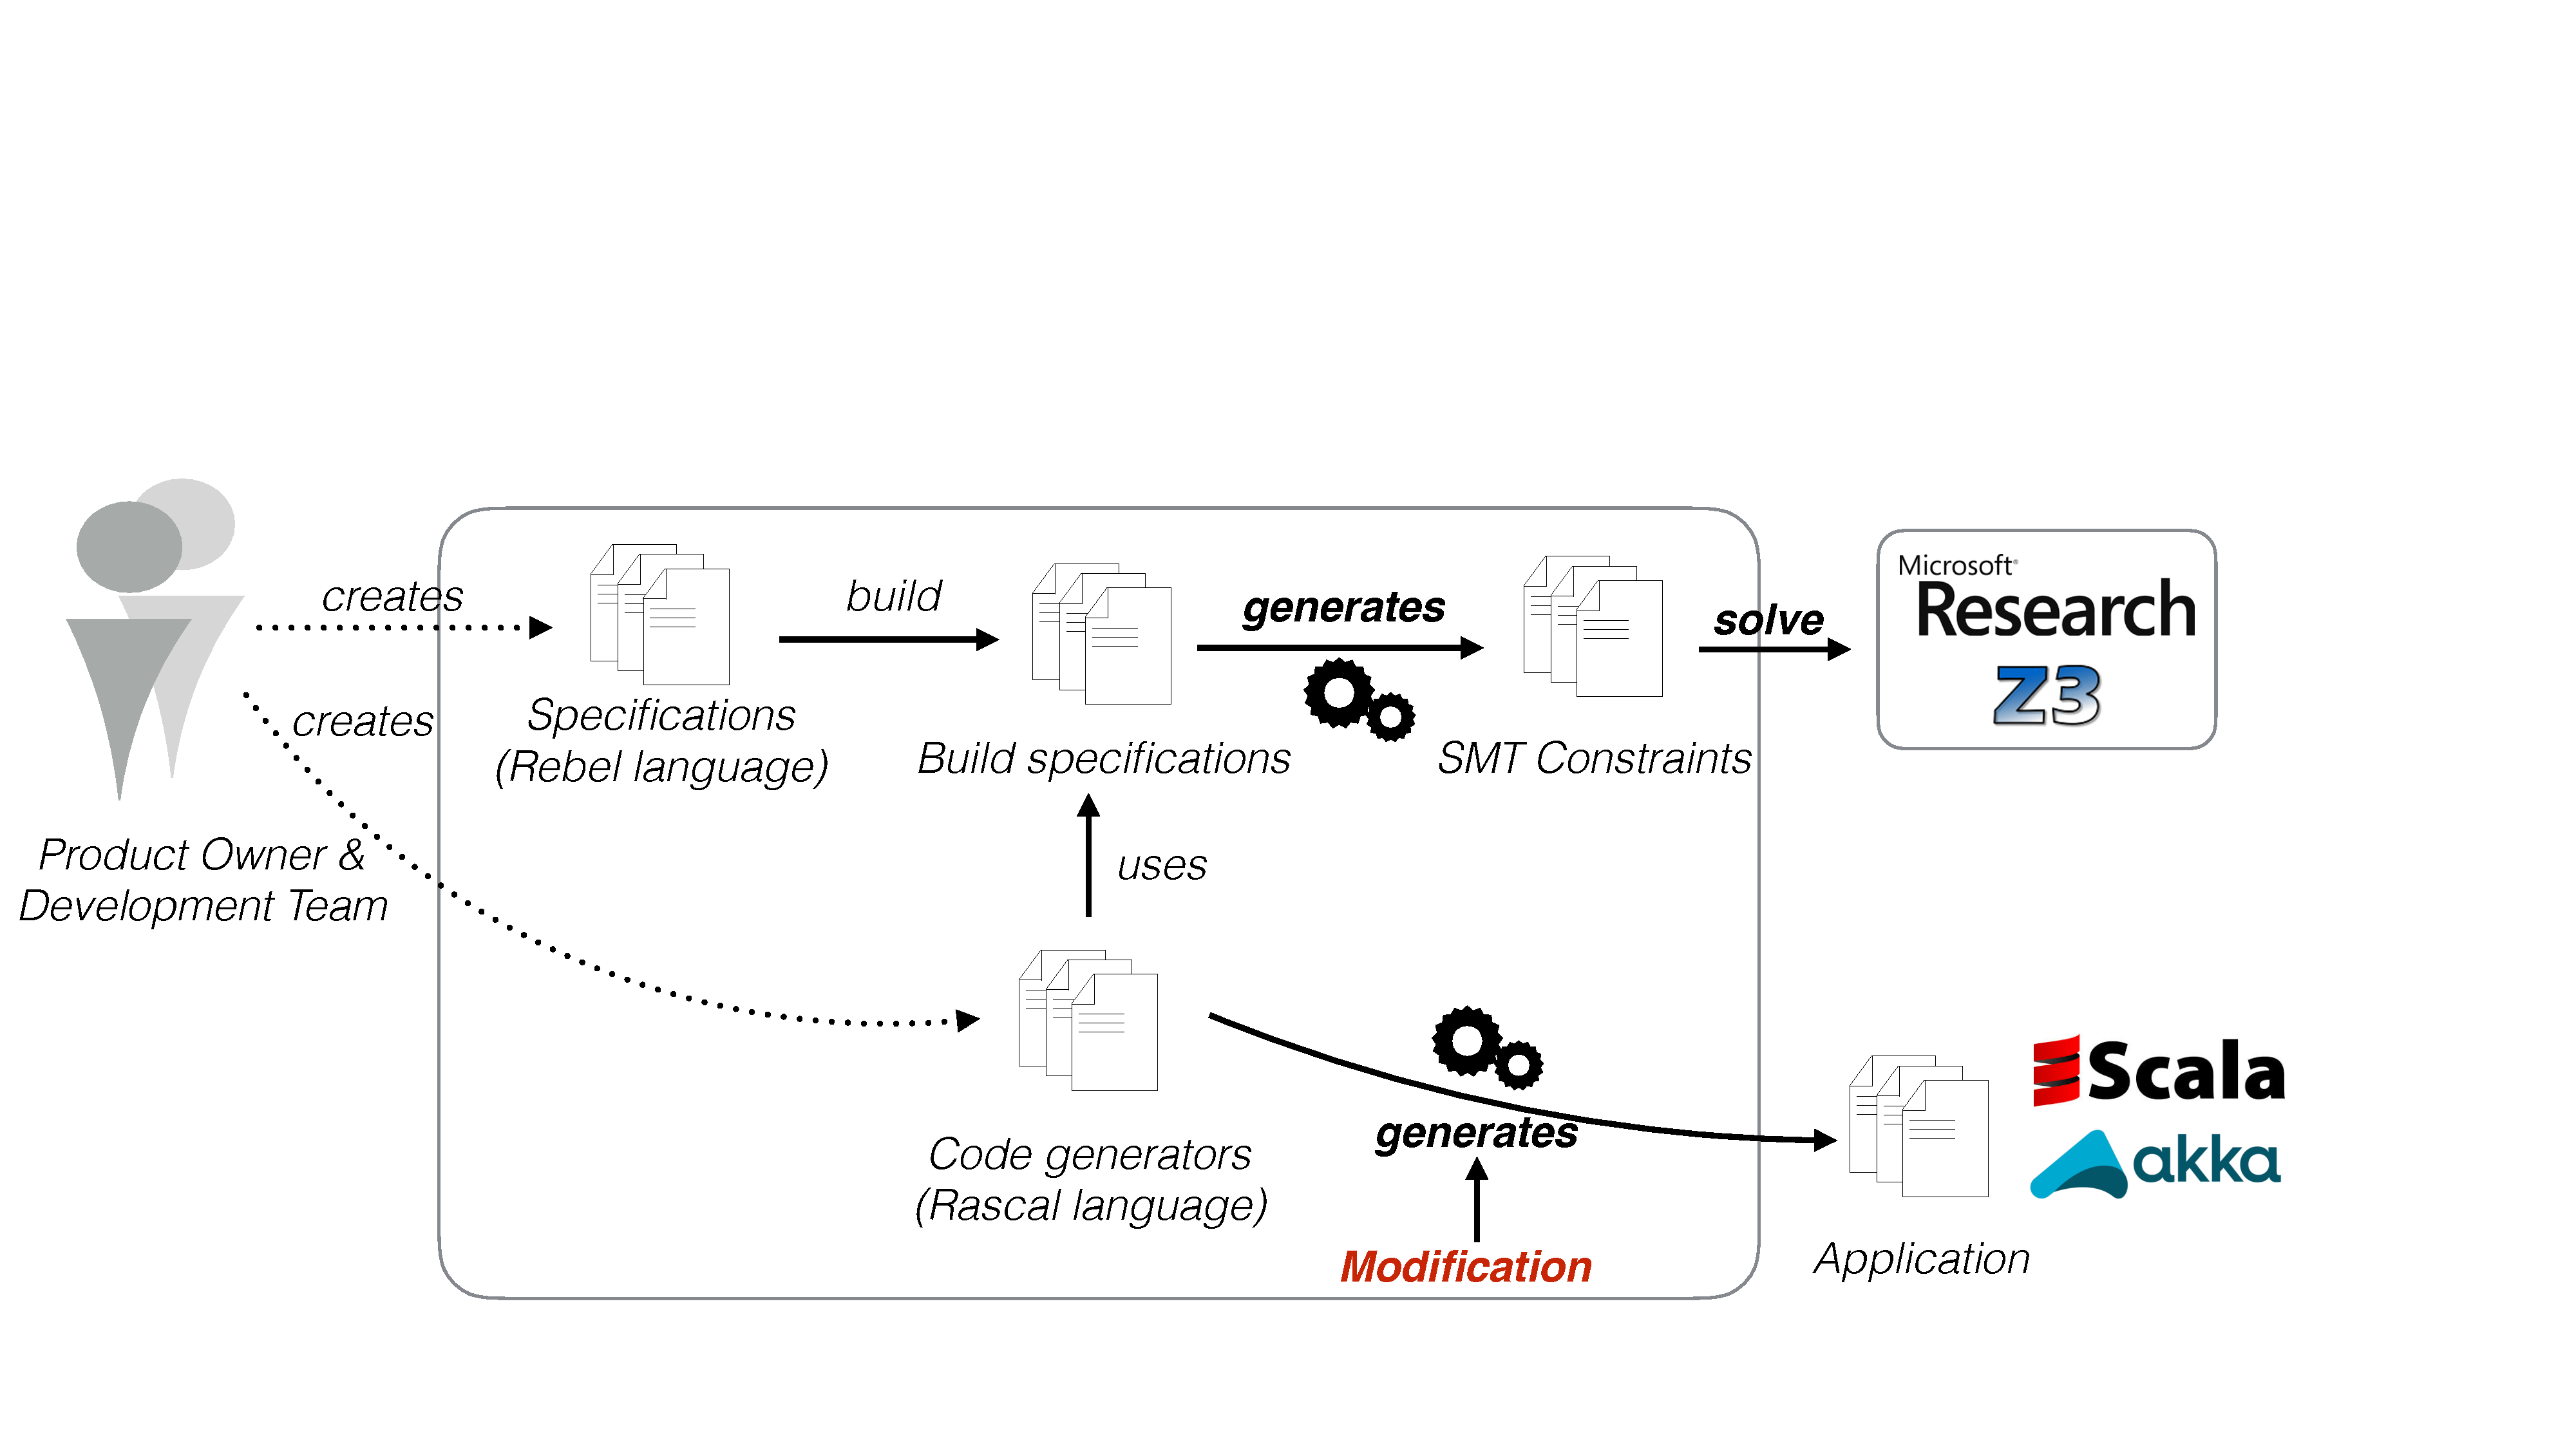
\includegraphics[scale=0.26]{figures/mod-generated.pdf}
  \caption{Modification in specification development}\label{fig:mod-spec-gen}
\end{figure}
\FloatBarrier

\begin{sourcecode}[h!]
\begin{lstlisting}[language=scala]
case Close() => {
  RebelConditionCheck.success
}
\end{lstlisting}
\caption{Modified Precondition for close event}\label{fig:account-close-mod-pre}
\end{sourcecode}
\FloatBarrier

Right now we have introduced a bug in the system under test (SUT), so the
generated system doesn't conform to the specification. We discussed earlier that
we are going to use the SMT solver to find bugs in the SUT.

Having an account with some balance in the state closed should not be possible
according to the specification. To let the SMT Solver solve this situation, it
is necessary to generate the appropriate SMT formulas. Therefore, checking can
be used to check whether the given state with its properties is reachable.

For this situation, is the following tebl file created, which is shown in
\autoref{fig:tebl-closed-account}. It defines the state of a closed account with
the property balance, where the balance isn't equal to zero. Also, here is 6
used as configurable time-out. The SMT solver tries to solve this problem in
max 6 steps.

\begin{sourcecode}[h!]
\begin{lstlisting}[]
module simple_transaction.ClosedAccountWithBalance

import simple_transaction.Account

state closedAccountWithBalance {
  closed Account with balance != EUR 0.00;
}

check closedAccountWithBalance reachable in max 6 steps;
\end{lstlisting}
\caption{Closed account test}\label{fig:tebl-closed-account}
\end{sourcecode}
\FloatBarrier

The input for the SMT solver is now defined. Similar behaviour should be defined
for the generated system. So an account needs to be opened and closed
afterwards.

The tebl file is passed to the model checker and it returns whether the given
SMT problem is reachable or not. A state is reachable when it can be reached
from the initial state via valid
transitions.~\cite[p.~4]{stoel_storm_vinju_bosman_2016} To check if the state is
reachable in the generated system, the request made for the given transition
contains afterwards a check whether the request is successful.

Since we've defined the input for both systems and are able to compare it, we
can trigger the bug and compare the results of it. As you can see in
\autoref{fig:result-trigger-one-bug}, the results of the model checker state
that the defined state in \autoref{fig:tebl-closed-account} isn't reachable and
that the state in the SUT is reachable.

\begin{sourcecode}[h!]
\begin{lstlisting}[]
rascal>check()

Reachable state false
Closed account true
bool: false
\end{lstlisting}
\caption{Results closing account comparison}\label{fig:result-trigger-one-bug}
\end{sourcecode}
\FloatBarrier

\section{Evaluation}\label{sec:ch3-evalution}
As we have seen with this lightweight version, it is able to find one specific bug with the use of an SMT Solver. Since the code generator is template based, it is possible to find faults in templating. There are two parts where there can occur faults during the generation parts. As first,~\cite[p.274]{voelter2013dsl} states that a majority of the generated code is fixed, some isolated parts are dependent on the input of the model. So it is possible that there might be bugs in the fixed code (skeleton). The second part is the template control code which is injected into the generated code. The manually introduced bug from the previous chapter belongs  to this category.

\unsure{\textbf{Onduidelijkheid DSL fowler}: styles of code generation: Model-Aware Generation and Model Ignorant Generation. Styles for generating textual output: Transformer
Generation and Templated Generation.}

\info{transactions, atomic commits, consistency. <- dit is moeilijk te doen. welke bugs verwacht je? het is moeilijk iets te generate. en uitleggen waarom het moeilijk is testen.}


%%%%%%%%%%%%%%%%%%%%%%%%%%%%%%%%%%%%%%%%%%%%%%%%%%%%%%%%%%%%%%%%%%%%%%%%%%%%%%%

% A little bit automated
\chapter{Experiment 1: Invalid execution traces}\label{sec:ch4}

The lightweight proof of concept discussed in \autoref{sec:ch3} is only able
to trigger one bug which is created manually. In this chapter, we discuss how
the lightweight proof of concept is automated and the test results of the
generated system.

\section{Method}

The lightweight version from the previous chapter is only able to test one specific
bug. The bug itself is created manually by modifying the \gls{sut}. Now,
this lightweight version needs to be automated to automatically generate a test
for every transition from a specification.

With every transition, it is possible to reach a state or stay in the current
state. To check \textit{Rebel} specifications, the state to reach with a transition needs
to be defined. As mentioned before, the goal of model checking is to find a
state which is reachable with some properties which do not hold
~\cite[p.~5]{stoel_storm_vinju_bosman_2016}. Thus defining only the reachable
state is not enough, the properties of interest for a transition needs to be
specified. Each property is different per transition, so these properties should
be different for the defined state. For example for the \textit{close}
transition, we want to check whether it is possible to have a closed account
where the balance is not equal to zero (as in \autoref{sec:ch3-method}),
for the transition \textit{withdraw} we want to check whether a negative balance
can be achieved with the transition. Again, with checking traces are not
available when a state is not reachable. In this case, traces cannot be used
with opposite preconditions since they are not provided.

To conclude, with this approach we are testing the opposite of the preconditions.
Thus what is not possible according to the specification is tested.

\subsection{Evaluation criteria}\label{sec:ch4-eval-criteria}

\subsubsection{Bugs}
Since we are testing with this approach the opposite of the preconditions, thus
what should be not possible according to the specification. It is expected to
find bugs in the \gls{sut} where it is possible to perform the opposite of a
transition. So faults can be found like preconditions which are not properly
generated. An example of this is the manually created bug
(\autoref{fig:ch3-res-codegenakka-account}) for the lightweight version.

\subsubsection{Efficiency}
In this approach is checking used to check what is not possible according to the
specification. Therefore, the same tested transition should be tested in the
\gls{sut}. To test all transitions from the account specification, it may take
longer since some transactions require an initial state for which transitions
need to be performed to reach this state.

\subsubsection{Coverage}
The experiment is going to generate a test for all transitions. Therefore,
it is expected to test all the transitions of a specification. With the criteria
bugs, we discussed the expectation to find faults in not properly generated
preconditions. This may lead to the inability to test transitions. For example,
when a failure (incorrect preconditions) occurs during reaching the initial
state of the \textit{withdraw} transition. This leads to the inability to test
the \textit{withdraw} transition.

\section{Approach}
The testing approach is a well-known approach in mutation testing. Mutation testing is
a fault-based testing technique, which generates faulty programs by syntactic
changes to the original program.~\cite[p.~1]{jia2011analysis} The set of faulty
programs are called mutants, each mutant contains a different syntactic change.
In our case, only one mutant is generated. A test suite for a program is used to
determine whether the faulty programs are detected. A mutant is killed when it
is detected by the test suite. The mutant is in our case killed when the result
from the \gls{smt} solver and the \gls{sut} are the same. we are using the same
approach from \autoref{sec:ch3} to compare the results of the \gls{smt} solver and
\gls{sut}.

Mutation testing generates a mutant based on
mutation operator, which is a transformation rule that generates a mutant from
the original program.~\cite[p.~3-4]{jia2011analysis} The mutation operator for
our approach is Negate Conditionals Mutator~\cite{pitmutators}, this operator
belongs to the type relational operator
replacement~\cite[p.~688]{king1991fortran}.

The testing approach is illustrated in \autoref{fig:mutated-checking}. The first
step is to start with a \textit{Rebel} specification, which is in our case the already
existing account specification. When the specifications are defined, the
specifications are being built, \textit{i.e.}, \gls{csts} are
produced of these specifications. Using these \gls{csts}, the code generator generates
the code, which is then the \gls{sut}.

The test case generator can be used to test the \gls{sut} when the \gls{sut} is generated
from the \gls{csts}. The \gls{csts} of the specifications are traversed by the test case
generator to generate a test for each transition. The test case generator
generates tebl files for transitions to use checking.

To test the \gls{sut}, the test case generator performs a similar transition
as used within checking in the \gls{sut}. Finally, the results from checking and the
performed transition in the \gls{sut} are compared.

\begin{figure}[h!]
  \centering
  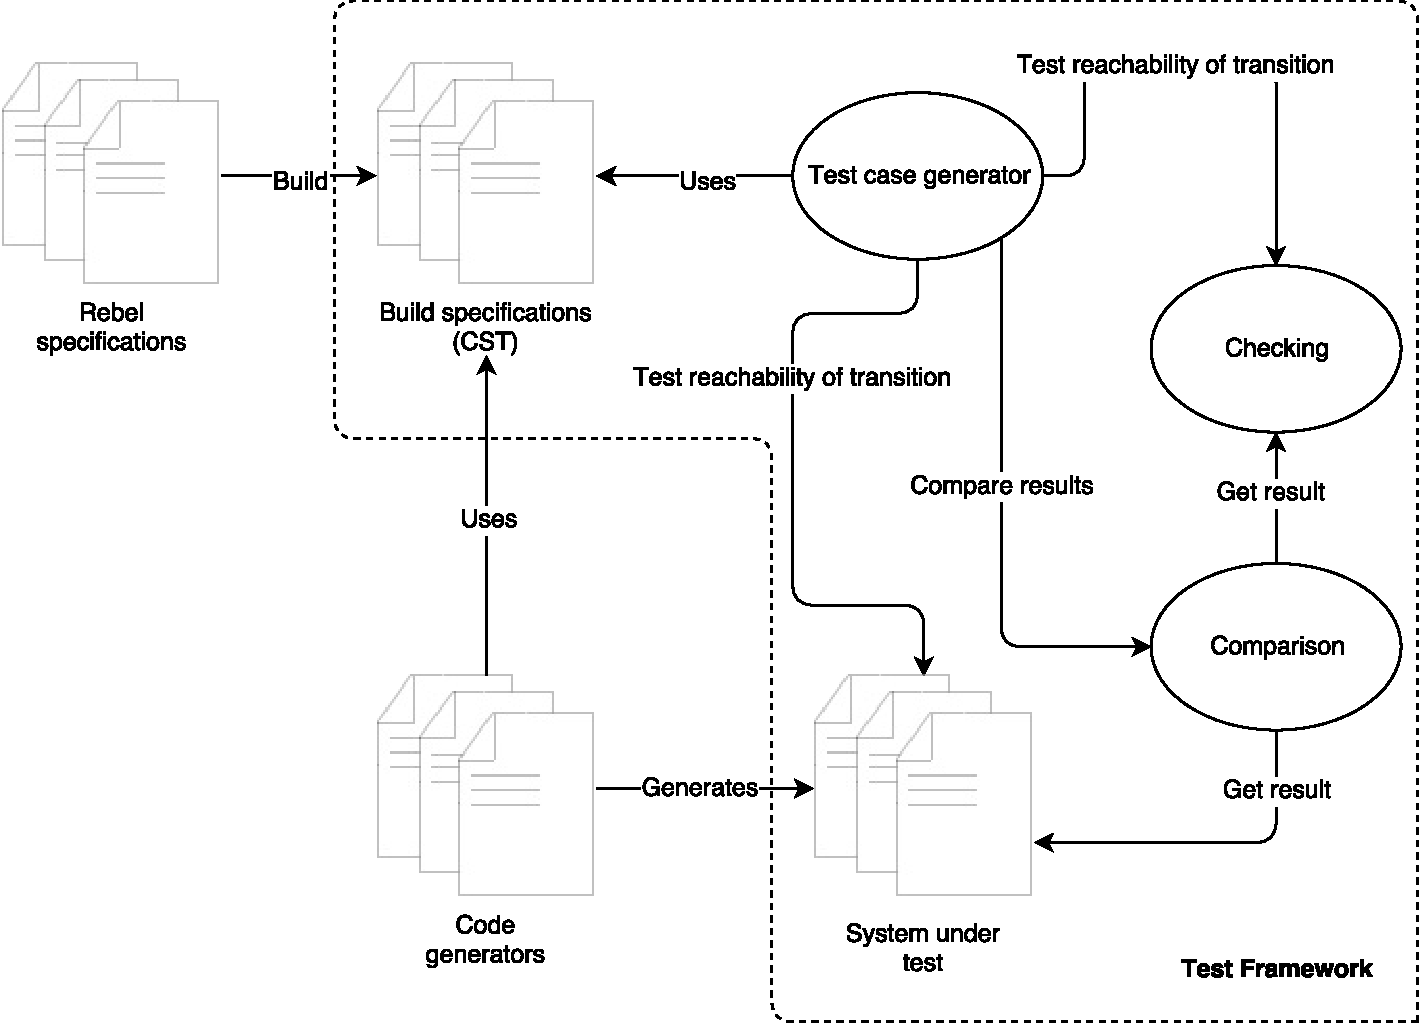
\includegraphics[width=\linewidth{}]{figures/mutated-checking-diagram.pdf}
  \caption{Testing approach with checking}\label{fig:mutated-checking}
\end{figure}
\FloatBarrier

\subsection{Checking}
Only expressions which contain a reference to the specification fields needs to
be replaced since it is only possible in tebl to specify the reachable state
with the properties of interest (these properties are not part of the
transition).

Earlier the definition of the \textit{close} event transition was given in
\autoref{fig:account-close-event} which contains the following statement
\code{this.balance == EUR 0.00;}. When this statement is translated to tebl
with a negated conditional, it looks as follows
\code{balance != EUR 0.00;}. Thus the replaced conditional is the opposite
condition of the statement defined in the \textit{close} transition.

Replacing conditionals to negated conditionals is done for all conditionals with
relational operators. The chosen mutation operator Negate Conditionals Mutator
will replace conditionals according to the replacement table in
\autoref{fig:table-replacement-conditions}.

\begin{table}[h!]
\centering
\begin{tabular}{cc}
\toprule
\textbf{Actual expression} & \textbf{Translated expression} \\ \midrule
!=                         & ==                             \\
==                         & !=                             \\
\textgreater               & \textless=                     \\
\textgreater=              & \textless                      \\
\textless                  & \textgreater=                  \\
\textless=                 & \textgreater                   \\ \bottomrule
\end{tabular}
\caption{Conditionals replacement~\cite{pitmutators}}\label{fig:table-replacement-conditions}
\end{table}
\FloatBarrier

\subsection{Generated system}
The conditionals for the transition in the \gls{sut} are also replaced.
Although, it is not necessary to replace always the conditionals. For some
transitions is an initial state required, \textit{e.g.}, to execute the transition unblock
of the account specification, the account should be in the state blocked. So an
initial state needs to be constructed for some transitions. Of course, the \gls{smt}
solver can construct its initial state to reach a state.

The definition of the \textit{deposit} transition is given in
\autoref{fig:account-deposit-event} and contains the following statement in the
preconditions \code{amount > EUR 0.00;}. First, the initial state needs to be
constructed which is the state opened. Following is the replacement of the conditionals, the
replaced precondition from the \textit{deposit} transition looks as follows
\code{amount > EUR 0.00;}. The \textit{deposit} transition needs then to be
performed in the \gls{sut}.

To perform the \textit{deposit} transition, the transition parameters for this
transition must be determined satisfying replaced conditionals. The transition
parameter for the \textit{deposit} transition, amount, should be less
than or equal to 0 euro. Therefore, are generators implemented to generate
values satisfying the negated conditionals. For example, the following
transition parameter is generated to be used in the \textit{deposit} transition
\code{"amount": "EUR -2.00"}.

\begin{sourcecode}[h!]
\begin{lstlisting}[]
event deposit(amount: Money) {
	preconditions {
		amount > EUR 0.00;
	}
	postconditions {
		new this.balance == this.balance + amount;
	}
}
\end{lstlisting}
\caption{\textit{deposit} event definition from specification}\label{fig:account-deposit-event}
\end{sourcecode}
\FloatBarrier

\section{Results}

\subsection{Codegen-Akka}

For this experiment, we are testing the generator Codegen-Akka. The results
of this test run are shown in \autoref{fig:ch5-res-codegenakka-account}. As shown
in this table, the tests for four transitions are successful and the tests for
the other three transitions are failed.

\begin{table}[h!]
\centering
\begin{tabular}{cc}
\toprule
\textbf{Transition to test} & \textbf{Transition} \\ \midrule
openAccount                 & \cmark{}            \\
withdraw                    & \xmark{}            \\
deposit                     & \xmark{}            \\
interest                    & \cmark{}            \\
block                       & \cmark{}            \\
unblock                     & \cmark{}            \\
close                       & \xmark{}            \\ \bottomrule
\end{tabular}
\caption{Results: testing account specification transitions}\label{fig:ch5-res-codegenakka-account}
\end{table}
\FloatBarrier

\section{Analyse}

\subsection{Codegen-Akka}

% https://github.com/cwi-swat/ing-rebel-generators/commit/999e6b40307a79fb245ace15375c27461c92374e
\subsubsection{Bug: closing an account with balance}\label{sec:bug-close-account}
When this automated version of checking is executed, it produces some false
positives. After investigating the tests for the transitions, the test for the \textit{close}
transition seems not be successful (see \autoref{fig:result-close-account}).
The model checker states that the state is not reachable (the same tebl file is
generated as in \autoref{fig:tebl-closed-account}). It seems to be that the
state is reachable in the \gls{sut}.

\begin{sourcecode}[h!]
\begin{lstlisting}[]
Test transition close
opened -> close -> closed
generated close test in |project://rebel-core/examples/simple_transaction/
  OpenedToClosedViaCloseTest.tebl|

Reachability transition: false
Execute transition result: true
Result successful transition test: false
\end{lstlisting}
\caption{Result run}\label{fig:result-close-account}
\end{sourcecode}
\FloatBarrier

When we take a look at the account in the \gls{sut}, it looks as
follows in \autoref{fig:closed-account-json}. The state of the account is in
closed, which is correct according to the specification, but the balance of the
account is 52 euro. In \autoref{fig:account-close-event} we already discussed
the event  definition of the \textit{close} transition, which is that the
balance should be equal to zero. From this, we can conclude that we have
discovered a bug in the \gls{sut}.

\begin{sourcecode}[h!]
\begin{lstlisting}[]
[{
	"_id": 17592186045441,
	"_version": 2,
	"_status": "CLOSED",
	"accountNumber": {
		"iban": "NO3627716652225"
	},
	"balance": {
		"value": 52.00,
		"currency": "EUR"
	}
}]
\end{lstlisting}
\caption{account state in json}\label{fig:closed-account-json}
\end{sourcecode}
\FloatBarrier

Now we know that we have discovered a bug, we want to know why this behaviour
occurs and whether it is due to the generated code from the specification. The
method which handles the \textit{close} transition has the following check in
\autoref{fig:java-notequal-check}. The if statement checks whether the balance
of the account is not equal to 0 euro. The condition in the if statement is not
satisfied with the balance of 52 euro. That is why the exception
\textit{BuildCASTransactionException} is not thrown.

\begin{sourcecode}[h!]
\begin{lstlisting}[language=Java]
if(! (isNotEqual(_entity.getBalance(), Money.of(org.joda.money.CurrencyUnit.of("EUR"), 0.00)))) {
  throw new BuildCASTransactionException("Predicate did not hold: CloseTransaction: this.balance ==
  EUR 0.00");
}
\end{lstlisting}
\caption{Code in Java}\label{fig:java-notequal-check}
\end{sourcecode}
\FloatBarrier

The question right now is, how is the above code generated. After taking a look at the synthesization of
expression, the expressions from \textit{Rebel} are not properly synthesized. The
synthesization for an equal expression for the type \textit{Money} or \textit{Percentage} looks as
follows in \autoref{fig:rascal-datomic-synthesize-equal}. The expression is
synthesized to the method \textit{isNotEqual} with two parameters.

\begin{sourcecode}[h!]
\begin{lstlisting}[]
private str g(e:(Expr)`<Expr lhs> == <Expr rhs>`, tmap t) = "isNotEqual(<g(lhs, t)>, <g(rhs, t)>)"
  when isType(t, lhs, (Type)`Percentage`) || isType(t, lhs, (Type)`Money`);
\end{lstlisting}
\caption{Generate equal expression in Rascal}\label{fig:rascal-datomic-synthesize-equal}
\end{sourcecode}
\FloatBarrier

So the expression is not properly synthesized, and it should be synthesized to
\textit{isEqual} instead of \textit{isNotEqual}. With this modification, it
is not possible anymore to close an account with some balance. This also applies
to other statements which use the equal operator.

% https://github.com/cwi-swat/ing-rebel-generators/pull/6
\subsubsection{Bug: deposit with a maximum amount}\label{sec:bug-compile-max-deposit}

The automated checking is implemented with the ability to first start the
\gls{sut} and then run the tests against it. For a new test run, the
specification has changed a little bit. It is now possible to only deposit with
a maximum amount (see \autoref{fig:java-deposit-maxamount}). After the code is
generated, the testing framework is not able to start the system. There is a
compile error as you can see in
\autoref{fig:java-result-lessthan-compile-error}, the binary operator "$<$"
is not applicable on the type \textit{org.joda.money.Money}. The compile error
is thrown by the source code from \autoref{fig:java-lessthan-compile-error},
which is part of the method which handles the \textit{deposit} transition.

% less than, not compilable. Duplicate method for greaterThan should be lessThan

\begin{sourcecode}[h!]
\begin{lstlisting}[]
event deposit(amount: Money) {
	preconditions {
		amount < EUR 250.00;
	}
	postconditions {
		new this.balance == this.balance + amount;
	}
}
\end{lstlisting}
\caption{\textit{deposit} event definition from specification}\label{fig:java-deposit-maxamount}
\end{sourcecode}
\FloatBarrier

\begin{sourcecode}[h!]
\begin{lstlisting}[]
Error:(63, 23) java: bad operand types for binary operator '<'
  first type:  org.joda.money.Money
  second type: org.joda.money.Money
\end{lstlisting}
\caption{\textit{deposit} event definition from specification}\label{fig:java-result-lessthan-compile-error}
\end{sourcecode}
\FloatBarrier

\begin{sourcecode}[h!]
\begin{lstlisting}[language=Java]
if(! ((amount < Money.of(org.joda.money.CurrencyUnit.of("EUR"), 200.00)))) {
  throw new BuildCASTransactionException("Predicate did not hold: DepositTransaction:
  amount < EUR 250.00");
}
\end{lstlisting}
\caption{Code in Java}\label{fig:java-lessthan-compile-error}
\end{sourcecode}
\FloatBarrier

The functions for the synthesization, which generates a part of
\autoref{fig:java-lessthan-compile-error}, are shown in
\autoref{fig:rascal-datomic-synthesize-lessthan}. Also here are the \textit{Rebel}
expression not properly synthesized. The default expression with the binary
operator "$<$" is properly synthesized to an expression with three expressions,
the left-hand and right-hand side expression and the binary operator "$<$".
As discussed before, the binary operator "$<$" doesn't work with
\textit{org.joda.money.Money}. Thus the default method to synthesize expressions
with the binary operator "$<$" cannot be used for the type
\textit{org.joda.money.Money}.

On line number 1 of \autoref{fig:rascal-datomic-synthesize-lessthan} is the
synthesization method of the expression with the binary operator "$>$" shown.
This method is already defined before in the corresponding file. To conclude,
this method should synthesize expressions with the binary operator "$<$".

\begin{sourcecode}[h!]
\begin{lstlisting}[]
private str g(e:(Expr)`<Expr lhs> \> <Expr rhs>`, tmap t) = "isGreaterThan(<g(lhs, t)>, <g(rhs, t)>)"
  when isType(t, lhs, (Type)`Percentage`) || isType(t, lhs, (Type)`Money`);
private str g(e:(Expr)`<Expr lhs> \< <Expr rhs>`, tmap t) = "(<g(lhs, t)> \< <g(rhs, t)>)";
\end{lstlisting}
\caption{Generate equal expression in Rascal}\label{fig:rascal-datomic-synthesize-lessthan}
\end{sourcecode}
\FloatBarrier

\section{Evaluation}\label{sec:ch4-evaluation}

\subsection{Bugs}
In \autoref{sec:ch4-eval-criteria} we discussed the expectations of the criteria
bugs. We expected to find bugs in the \gls{sut} where it is possible to perform
the opposite of a transition. Thus it is expected to find bugs where the
preconditions are not properly generated.

With this experiment, we have found a bug in the \gls{sut}, which was
discussed in \autoref{sec:bug-close-account}. The other bug is out of scope
since the \gls{sut} is not able to compile. With the bug from
\autoref{sec:bug-close-account}, it is possible that the final state closed is
reached where the preconditions of the \textit{close} transition do not hold.
So as expected, we did find a bug in performing the opposite of a transition
where the preconditions were not properly generated.

In this experiment traces are not used because they cannot be provided by the
\gls{SMT} solver when a state is not reachable. The expectation is that with
testing the opposite preconditions, not reachable states, traces are not
provided. Remarkable is that with testing some transition, the traces are
provided, because the state to reach with checking are reachable. For example,
the \textit{block} transition has no precondition which means that the state to
reach is reachable with checking.

\subsection{Efficiency}
For the criteria efficiency, it is expected to check what is not possible
according to the specification, i.e. testing the same transition in checking as
well as in the \gls{sut}.

A part of the generated test for a transition is checking, which is used to test
the state to reach with the replaced preconditions. So, in this experiment, we
are testing what should be not possible according to the
specification. The expectation is that the same transitions with checking should
be performed on the \gls{sut}. However, the result of the checking from the
\gls{smt} solver varies, \textit{e.g.}, an opened account can be reached by the
\textit{openAccount} transition or by the transition \textit{openAccount} and
\textit{withdraw}. Thus the test framework is not able to perform the same
transitions on the \gls{sut} as the transitions from checking.

With testing all transitions from the account specification, it is possible that
testing may take longer. As expected, this is the case since due to the initial
state transitions are more executed and tested. To conclude, the testing process
may take longer to test all the transitions.

\subsection{Coverage}
It is expected for this criteria to test all the transitions of the
specification since the experiment generated tests for all transitions.

In the experiment, after the checking, a transition
is performed in the \gls{sut}. In this experiment, it is unknown whether the
performed transition with its parameters in the \gls{sut} is the same as the
transition computed by the \gls{smt} solver. This causes some false positives in the
test run. Also, it is difficult to play like the \gls{smt} solver; it is unknown which
result the \gls{smt} solver will give. The \gls{smt} solver is also smarter/better in checking
the satisfiability of a given constraints.

Failure occurring along the way in constructing the initial state of a transition
may lead to the inability to test transitions. Unfortunately, there does not
seem to be any faults in here.

\section{Conclusion}
In this experiment is the account specification used to test the \gls{sut}.
This experiment generates automatically tests for transitions.

A part of
the generated test for a transition is checking, which is used to test the state to
reach with the replaced preconditions. So, in this experiment, we are
testing what should be not possible according to the specification. The result
of the checking from the \gls{smt} solver varies, \textit{e.g.}, an opened account can be
reached by the \textit{openAccount} transition or by the transition
\textit{openAccount} and \textit{withdraw}.

After the checking, a transition
is performed in the \gls{sut}. In this experiment, it is unknown whether the
performed transition with its parameters in the \gls{sut} is the same as the
transition computed by the \gls{smt} solver. This causes some false positives in the
test run. Also, it is difficult to play like the \gls{smt} solver; it is unknown which
result the \gls{smt} solver will give. The \gls{smt} solver is also smarter/better in checking
the satisfiability of a given constraints.

To conclude, the checking used in this experiment tests only the states, regardless of which transitions are
being performed, and testing the \gls{sut} focuses more on testing transitions.

With this experiment, we have found a bug in the \gls{sut}, which was
discussed in \autoref{sec:bug-close-account}. The other bug is out of scope
since the \gls{sut} is not able to compile. The found bug belongs to the category
injected code since the generated code for the precondition is wrong. In this
case, the final state closed is reached where the preconditions of the \textit{close}
transition do not hold.

% So the theory for this found bug is
% $\forall e s_{1} \to s_{2}, s_{2} \gets s_{1}, pre(e)$.

% claims from finding the bugs.

% \begin{itemize}
% \item je bent in een state gekomen via een preconditie
% \item de transitie zelf verander de pre conditie niet, (de preconditie geldt dan in de postconditie)
% \item het was de laatste

% \item $\forall e s1 \to s2, in s2 geldt pre(e) \lor (! pre(e) \land post(e))$
% \item $\forall e s1 \to s2, in s2 post(e)$
% % of?
% \item $\forall e s1 \to s2, s2 alleen bereikbaar via (1), dan pre(e)$
% \end{itemize}

\section{Threats to validity}

\subsection*{Limited specifications}
In the conducted experiment is the account specification account used
to test the \gls{sut}. With this experiment and specification,
we did find a bug in the code generators.

The used account specification in this experiment is quite simple. With the use
of more interacting specifications, the chance is bigger to find faults in the code
generators since the specifications are interacting with each other.

\subsection*{Invalid execution trace}
The conducted experiment test only what should be not possible according to the
specification. It is also important to test whether the \gls{sut} is conform to the
specification, \textit{i.e.}, testing the valid execution trace.


%%%%%%%%%%%%%%%%%%%%%%%%%%%%%%%%%%%%%%%%%%%%%%%%%%%%%%%%%%%%%%%%%%%%%%%%%%%%%%%

% Simulation
\chapter{Checking \& Simulation}
\label{sec:ch5}

In this chapter, we discuss how to solve the limitations of the previous
approach and how to solve them by using the simulator.

\section{More complex specifications}
In the previous approaches is only the account specification used. In this proof
of concept, we're going to use more complex specifications, complex in the sense
that they depend and interact with each other. Therefore, we're going to use the
same account specification from \autoref{fig:account-spec}. As an addition to
account specification, we use a transaction specification. Via this
specification money can be transferred between two accounts.
The Rebel implementation of the transaction is shown in
\autoref{fig:transaction-spec} \footnote{\url{https://github.com/cwi-swat/rebel/blob/e58590c7f51f59e7ee6443bb89ef09dff6febab6/rebel-core/examples/simple_transaction/Transaction.ebl}}.
As you can see the transaction specification contains more fields than the
account specification. The two remarkable fields are from and to, both are the
type of IBAN \info{ref paper}. Note that after the type definition an annotation
is given to specify a reference to another specification, in this case, account
specification. The fields to and from are used to indicate between whom the
transaction takes place. According to the specification, the transaction first
needs to be started. When a transaction is in the state validated and booking
cannot be made, the transition fail can be used to put the transaction in its
final state failed. To successfully complete a transaction is the transition
book used. In comparison to the account specification, does the transaction
specification two final states, which are booked and failed. When the final
state booked or failed is reached, then there is no further action allowed.
Note that the transaction specification doesn't have an invariant.

Another difference in the transaction specification is that event definitions
can contain sync expressions. From the previous event definitions, we've only
seen pre- and postconditions. Sync expressions are used for synchronization.
These sync expressions are also translated to SMT formulas. These sync
expressions translated to the SMT Solver are just logical formulas, there is no
logic for synchronization in these formulas. Of course, the generated system has
implemented synchronization for these transitions. So it is possible to also
test synchronization in the SUT. There are also several studies which reports
that SMT-based approaches to model checking can be used to test distributed
algorithms \cite{konnov2015you,alberti2015smt}.
% Sync expressions are used to synchronously execute a blocking transition without the interference of other related transitions which may change the state of the instances used within the sync expressions. \unsure{which is better? or a paper ref?}
The block transition uses this feature to express sync operations (see
\autoref{fig:transaction-book-event}). A sync operation is here used to withdraw
an amount from one account and to deposit to another account.

\info{new scala generator, two-phase commit for distribution.}
\info{explain sync stuff and about distribution, look at implementation of
sync in smt. Theoretically it is possible to find errors in distributed stuff.}

\begin{sourcecode}[h!]
\begin{lstlisting}[]
specification Transaction {
	fields {
		id: Integer @key
		amount: Money
		from: IBAN @ref=Account
		to: IBAN @ref=Account
	}

	events {
		start[]
		book[]
		fail[]
	}

	lifeCycle {
		initial uninit -> validated: start
		validated    -> booked: book
					-> failed: fail
		final booked
		final failed
	}
}
\end{lstlisting}
\caption{Transaction specification}
\label{fig:transaction-spec}
\end{sourcecode}

\begin{sourcecode}[h!]
\begin{lstlisting}[]
event book() {
	sync {
		Account[this.from].withdraw(this.amount);
		Account[this.to].deposit(this.amount);
	}
}
\end{lstlisting}
\caption{book event definition from transaction specification}
\label{fig:transaction-book-event}
\end{sourcecode}

\section{Method}
% The simulation of Rebel is able to translate a single step to SMT formulas.

As discussed in \autoref{sec:research-method}, a model testing approach is
already done to test existing banking systems. Although, in this approach, it
was only possible to test the SUT interactively using the simulation. The traces
are used to check whether the SUT accepts the execution from the trace and
whether it behaves as the specification.~\cite[p.5]{stoel_storm_vinju_bosman_2016}
In addition, with the use of traces, it solves also the problems from the
previous chapter, we know exactly what is done by the SMT and playback it in the
SUT. Therefore, we're going to use the traces in this approach to check the
behaviour of the SUT.

\subsection{Evaluation points}
Evaluation points and expectations.

\section{Approach}
It is possible that a trace can contain multiple steps, \textit{e.g.}, to
unblock an account, an account needs first to be opened and blocked. To playback
the steps from a given trace on the SUT, we're going to split every transition
into three steps as in ~\cite{stoel_storm_vinju_bosman_2016}:
\begin{enumerate}
\item \textbf{pre-transition check} Check whether the current state from the SUT
is conform to the current state from the trace
\item \textbf{transition check} Execute the given transition from the trace on
the SUT
\item \textbf{post-transition check} Check whether the new state from the SUT is
conform to the new state from the trace
\end{enumerate}
\unsure{paper: what is state? also the values of the instances?}

The transition function for the simulation looks as follows: $p(s_{1}, s_{2})$,
which has the pre- and postcondition of the to be executed transition
\cite[p.6]{stoel_storm_vinju_bosman_2016}. The current state $s_{1}$ holds the
constraints of the current values of the simulated specification. Hereafter, to
execute the transition the user is asked to provide the data for the transition
parameters. Before we can use the simulation, solve two things: current state,
user feedback. User feedback isn't relevant in this case since it needs to be
automated. These problems are discussed in the paragraphs below.

\subsection{Pre-transition check}

\subsubsection*{Current state}
\label{sec:ch5-current-state}

The pre-transition checks entail the check for the current state of the SUT is
conform to the current state from the trace. Although with the simulation it is
only possible to reason about individual steps. For some transitions a current
state is required, \textit{e.g.}, an account needs to be blocked first to
unblock it. In the simulation, a current state needs to be defined to check
whether the step can be made from the current state. This is also the case in
the SUT since a current state needs to be initialized first before the
transition is made.

To initialize the current state in the SUT checking can be used. By defining
the current state with checking, it is checked and return a valid trace when
it is satisfiable. So for every transition, a tebl needs to be generated for the
state to reach (current state) to perform the transition. Although there are a
number of caveats with the use tebl files.

When a state to reach is defined for checking, the identifiers for the entities
are only unique within that trace. For example for
\autoref{fig:tebl-opened-simple-account}, the identifier for the opened account
from the traces is \textit{NL10INGB0000001}. The identifiers for similar
entities are auto-incremented, \textit{e.g.}, when an additional account entity
is specified in \autoref{fig:tebl-opened-simple-account} the identifier is then
\textit{NL10INGB0000002}. This is not only the case with IBAN numbers but also
with Integer, String, etc. This isn't a problem when a single transition is
tested, but when multiple transitions are tested when there are multiple
entities, this will result in collisions of existing entities with the same
identifiers. Note also that the generated IBAN numbers by the SMT Solver are
also not valid. \improvement{why? representation of iban in smt. String pooling
stuff, for the smt stuff.} The invalid IBAN numbers isn't a problem for the
checking since checking is only used to reason about possible traces. However,
this doesn't hold in the SUT, since SUT is a banking system and here it must
conform to the IBAN standards. It is possible with checking to define the
properties of an entity, \textit{e.g.}, the IBAN for an account. To solve the
problem with the collision of existing entities, a random identifier should be
given for each entity. Therefore, for each type like Integer, is a simple random
generator implemented. This generator generates a random identifier which is
used as the identifier for the entities in checking. Unlike the basic types,
IBAN is a more complex type to generate since the type should conform to the
IBAN standards. Therefore, Iban4j \footnote{\url{https://github.com/arturmkrtchyan/iban4j/tree/ce1ca12b947755d1d96aab294d1ea15c78090ca2}}
is used to generate random IBAN account numbers which are compliant to the
ISO\_13616 ISO\_9362 standards.

Another pitfall with the use of checking is the use of more complex
specifications, \textit{e.g.}, the transaction specification. With such
specifications, it is possible to have a reference to another specification. In
the case of the transaction specification involves two references, namely
account specification. To use checking in such specifications must be taken into
account the references to other specifications. Which means that for every
referencing specification in checking, imports need to be resolved and defined,
and the entity needs to be defined with an identifier. Note that these
identifiers should be again random, otherwise it will cause again collisions of
existing entities.

Altogether, a generated tebl for checking the current state looks as follows in
\autoref{fig:tebl-gen-validated-transaction}.

\begin{sourcecode}[h!]
\begin{lstlisting}[]
module simple_transaction.Test

import simple_transaction.Transaction
import simple_transaction.Account


state doCheck {
  validated Transaction with id == 65227;

  Account with accountNumber == NO3631174980518;
  Account with accountNumber == LB404150J311SB1FJV5KL1MKYAY4;
}

check doCheck reachable in max 6 steps;
\end{lstlisting}
\caption{Generated tebl for the transition book}
\label{fig:tebl-gen-validated-transaction}
\end{sourcecode}

\subsubsection*{Current state values}
After the current state is defined, the same approach from the previous chapter
can be used to check whether it satisfiable. The SMT Solver returns whether it
is satisfiable with the traces, including instances with its values. The last
step is taken and the instances from here. The values from these instances of
the simulated specifications are given to the current state $s_{1}$
\improvement{why?}.

The simulation checks only whether the step can be made from the given current
state, it doesn't check whether the current state is reachable. With the use of
checking for the current state,


There is also reason to argue if this is possible



Execute traces against generated system to have the instances initialized. This
is in more depth described in chapter traces. Each step within a trace is a
transition, so test this every three steps.

\subsection{Transition check}
% Execute the given transition from the trace on the SUT

\subsubsection*{Transition parameters data values}
Since simulation is used for reasoning about individual steps, that explains why
the transition parameters data values for the chosen transition should be
provided by the user. And as discussed earlier is in the model testing approach
of the study \cite[p.6]{stoel_storm_vinju_bosman_2016} chosen for interactively
using the simulation. Manually providing the transition parameters data values
isn't relevant for us, since our intention is to test automatically the SUT.
Certainly, these values can be generated randomly, but it should satisfy the
given pre- and postconditions for the chosen transition. However, it would be
better to let the SMT solver fill these values, taking into account the pre- and
postconditions of the chosen transition. At the time of the publication of the
\cite{stoel_storm_vinju_bosman_2016}, this wasn't possible in the simulation, so
the simulation should be slightly modified.

In cooperation with the author is this feature added to the simulation.
\footnote{\url{https://github.com/cwi-swat/rebel/commit/0d29eb30a82cc5dd6d8be750daa4a24e4e2786be}}
The simulation is now able that both state variables and transition variables
can be left open, in the sense of using the expression \textit{ANY}. When the
expression \textit{ANY} is used, the SMT solver will fill in a value for the
corresponding transition parameter, satisfying the pre- and postconditions for
the chosen transition. \unsure{what about expression as iban?}

\subsubsection*{Traces}
A valid trace is a chain of valid transitions from one state to the next state
\cite[p.5]{stoel_storm_vinju_bosman_2016}. The trace may contain multiple steps,
each step has instances with its state and values. These instances are specific
for that step, the results after performing the step are given in the state and
values for an instance. A trace for simulation contains the state before
performing the transition, the step (transition), and then the state after
performing the step.

After everything is defined for the simulation, the simulation can test whether
it can make the single step. The simulation then works as follows
\cite[p.6]{stoel_storm_vinju_bosman_2016}:
\begin{enumerate}
\item Whether it is possible to satisfy the constraints of the selected events
given the current state and actuals of the transition parameters of the event:
$p(s_{1}, s_{2})$
\item Whether the invariants (the safety property) hold in the resulting state:
$P(s2)$.
\end{enumerate}

When this step can be made, with the use of traces, the step can be played in
the SUT. Therefore, \textit{JSON} should be generated for the chosen transition.
To generate this \textit{JSON} are the transition parameters data values and
the transition name read from the trace step. At last, the endpoint is
determined for the given step and is the generated JSON sent to the endpoint.

\subsection{Post-transition check}
% Check whether the new state from the SUT is conform to the new state from the trace

Since a trace contains the instances before and after the step, this can be used
in the post-transition check to test the SUT. As a result, we can check after or
before performing the step, whether the SUT behaves similarly as the
simulated/checked specification. To check whether the new state from the SUT is
conform to the trace, the state and values from the instances are read after
performing the transition. The endpoint is then determined to retrieve the state
of these instances in the SUT. Then, the results of these instances from the SUT
and trace are compared to find any misbehaviour in the SUT.
\improvement{check all instances}

Before a Rebel specification is checked or simulated is the specification
normalized. This normalization process is done to make the SMT formulas easier
and also to give it partially semantics
\cite[p.5]{stoel_storm_vinju_bosman_2016}. Desugaring the life cycle is part of
the normalization process. The life cycle is desugared to strengthen the pre-
and postconditions of the transitions with the life cycle information.
Therefore, are two fields added, \_state and \_step, to the fields of the
specification. To each state and event is a distinct identity assigned. The
identity of the current state is assigned to the \_state field and the identity
of the transition which led to the current state is assigned to the field
\_step. This results into that the original life cycle can be expressed, by
adding constraints on the \_state and \_step fields to the transitions pre- and
postconditions \cite[p.5]{stoel_storm_vinju_bosman_2016}. The newly added fields
are also present within the trace from the SMT Solver. In our case, we only use
the \_state field, because we already know which transition let to the current
state. To compare the current state from the \_state field, it needs to be
sugared back in order to compare it to the SUT.
% Adding Frame Conditions. To guard the fields that are not changed by the event frame conditions are added (Jack- son 2012). These frame conditions make sure that a field has the same value after the transition as before.

As discussed in the code generation section, the request made to the API of the
SUT are "standardized", but the response isn't. For the post-transition check,
it is necessary to check the new state in the SUT, and therefore an adapter
needs to be defined to be able to compare the results of the SUT and the trace.
The decision is made to only implement an adapter for the code generator
Codegen-Akka, since this is a more mature code generator and frequently used for
experiments within ING Bank.

% Using the generated test cases, we can then test the system. Usually, an adapter is used to decouple knowledge of the SUT’s external interfaces from the test generation tool. The test cases provide the inputs and expected outputs to the adapter. The adapter forwards the inputs to the SUT. When the SUT sends a response, the adapter observes it and evaluates it using the expected outputs

% as discussed with current state, all transitions contains the tree steps. It is possible that a trace can contain multiple steps, e.g. to unblock an account, an account needs first to be opened and blocked. This requires after executing each step, the step needs to be tested, in the sense of automatically repeating the process.

\section{Results}
Discuss the results of the test approach.

\subsection{Codegen-Akka}

\begin{table}[h!]
\centering
\begin{tabular}{ccc}
\toprule
\textbf{Transition to test} & \textbf{Current state} & \textbf{Transition} \\ \midrule
openAccount                 & \cmark{}               & \cmark{}            \\
withdraw                    & \cmark{}               & \cmark{}            \\
deposit                     & \cmark{}               & \cmark{}            \\
interest                    & \cmark{}               & \cmark{}            \\
block                       & \cmark{}               & \cmark{}            \\
unblock                     & \cmark{}               & \cmark{}            \\
close                       & \cmark{}               & \xmark{}            \\ \bottomrule
\end{tabular}
\caption{Results: testing account specification transitions}\label{fig:ch5-res-codegenakka-account}
\end{table}

\begin{table}[h!]
\centering
\begin{tabular}{ccc}
\toprule
\textbf{Transition to test} & \textbf{Current state} & \textbf{Transition} \\ \midrule
start                       & \cmark{}               & \cmark{}            \\
book                        & \cmark{}               & \cmark{}            \\
fail                        & \cmark{}               & \cmark{}            \\ \bottomrule
\end{tabular}
\caption{Results: testing transaction specification transitions}\label{fig:ch5-res-codegenakka-transaction}
\end{table}

\subsection{Codegen-Datomic}

\begin{table}[h!]
\centering
\begin{tabular}{ccc}
\toprule
\textbf{Transition to test} & \textbf{Current state} & \textbf{Transition} \\ \midrule
openAccount                 & \cmark{}               & \cmark{}            \\
withdraw                    & \cmark{}               & \cmark{}            \\
deposit                     & \cmark{}               & \cmark{}            \\
interest                    & \cmark{}               & \xmark{}            \\
block                       & \cmark{}               & \cmark{}            \\
unblock                     & \cmark{}               & \cmark{}            \\
close                       & \cmark{}               & \xmark{}            \\ \bottomrule
\end{tabular}
\caption{Results: testing account specification transitions}\label{fig:ch5-res-codegendatomic-account}
\end{table}

\begin{table}[h!]
\centering
\begin{tabular}{ccc}
\toprule
\textbf{Transition to test} & \textbf{Current state} & \textbf{Transition} \\ \midrule
start                       & \cmark{}               & \cmark{}            \\
book                        & \cmark{}               & \cmark{}            \\
fail                        & \cmark{}               & \cmark{}            \\ \bottomrule
\end{tabular}
\caption{Results: testing transaction specification transitions}\label{fig:ch5-res-codegendatomic-transaction}
\end{table}

\subsection{Codegen-Scala-ES}

\begin{table}[h!]
\centering
\begin{tabular}{ccc}
\toprule
\textbf{Transition to test} & \textbf{Current state} & \textbf{Transition} \\ \midrule
openAccount                 & \cmark{}               & \cmark{}            \\
withdraw                    & \cmark{}               & \cmark{}            \\
deposit                     & \cmark{}               & \cmark{}            \\
interest                    & \cmark{}               & \xmark{}            \\
block                       & \cmark{}               & \cmark{}            \\
unblock                     & \cmark{}               & \cmark{}            \\
close                       & \cmark{}               & \xmark{}            \\ \bottomrule
\end{tabular}
\caption{Results: testing account specification transitions}\label{fig:ch5-res-codegenscalaes-account}
\end{table}

\begin{table}[h!]
\centering
\begin{tabular}{ccc}
\toprule
\textbf{Transition to test} & \textbf{Current state} & \textbf{Transition} \\ \midrule
start                       & \cmark{}               & \cmark{}            \\
book                        & \cmark{}               & \cmark{}            \\
fail                        & \cmark{}               & \cmark{}            \\ \bottomrule
\end{tabular}
\caption{Results: testing transaction specification transitions}\label{fig:ch5-res-codegenscalaes-transaction}
\end{table}

\section{Analyse}
Analyse of the results

\subsection{Codegen-Akka}
The proof of concept uses in this test run the Codegen-Akka generator.
Investigating the test run, it seems to be that all transitions are tested
successfully, except the transition \textit{close}. Also, there seems to be a
limitation in testing the state of a specification.

\subsubsection{Close transition}
\label{sec:close-no-test-codegenakka}

The result of \textit{close} transition test is shown in
\autoref{fig:result-codegenakka-close}. As you can see on line number 28 is
constructing the current state for the close transition successful. Then the
simulation is asked to simulate the close transition, but according to the
traces of the simulation, the simulation wasn't able to make the step and the
simulation returns only the state before the transition.

\begin{sourcecode}[h!]
\begin{lstlisting}[]
Test transition close
opened -> close -> closed

0:
  now = 14 Aug 2017, 13:49

  instance: simple_transaction.Account, key = FO9402337176862639
    ?
    ?
    var accountNumber (type: IBAN) (uninitialized)
    var balance (type: Money) (uninitialized)

1:
  now = 14 Aug 2017, 13:49
  step: simple_transaction.Account.openAccount
    var initialDeposit (type: Money) = EUR50.00
    Transition to state = opened
    Identified by accountNumber = FO9402337176862639

  instance: simple_transaction.Account, key = FO9402337176862639
    State = opened
    ?
    var accountNumber (type: IBAN) = FO9402337176862639
    var balance (type: Money) = EUR50.00

Endpoint: /Account/FO9402337176862639/OpenAccount
JSON payload: { "OpenAccount": { "initialDeposit":"EUR 50.00" } }
Response: ("body":"CommandSuccess(OpenAccount(50.00 EUR))","isSuccessful":"true","message":"OK",
"errorBody":"","code":"200")

1:
  now = 12 Jul 2016, 12:00:00

  instance: simple_transaction.Account, key = FO9402337176862639
    State = opened
    ?
    var accountNumber (type: IBAN) = FO9402337176862639
    var balance (type: Money) = EUR50.00
\end{lstlisting}
\caption{No test generated for close transition}
\label{fig:result-codegenakka-close}
\end{sourcecode}

As discussed earlier, the precondition of the close transition is that there
should be no remaining balance as shown in \autoref{fig:account-close-event}.
On line number 15 of the test run is shown that the simulation makes the step to
open an account with a balance of 50 euros. Afterwards are no transitions
performed. Thus this current state does not satisfy the precondition of the
close transition. That's why the simulation wasn't able to perform the
transition since the given values from the current state to $s_{1}$ weren't
satisfying for $s_{2}$. The generated tebl for the current state is shown in
\autoref{fig:tebl-gen-validated-transaction}. Only the state to reach is
specified with the identifier of the account. As we've seen the event definition
of \textit{openAccount} in \autoref{fig:account-openaccount-event}, the account
must be opened with a balance of 50 euros.
To conclude, the simulation wasn't able to test the transition close since the
precondition of this transition isn't satisfied in the postcondition of $s_{1}$.

\begin{sourcecode}[h!]
\begin{lstlisting}[]
module simple_transaction.Test

import simple_transaction.Account

state doCheck {
  opened Account with accountNumber == AD3517248539N3OTXZIDF13H;
}

check doCheck reachable in max 6 steps;
\end{lstlisting}
\caption{Generated tebl for the transition book}
\label{fig:tebl-gen-validated-transaction}
\end{sourcecode}

\subsubsection{State testing}

In \autoref{fig:result-not-found-state} is the test run shown of the transition
\textit{book}. Only the first transition is shown in this figure. As you can
see on line 42 is the \textit{openAccount} transition performed. On the line
below is shown that the request is successful. On line 44 is an error message
shown which tells that it isn't able to find the state of the opened account.
Note the question mark in this message. This error message is part of the
post-transition check where the new state of the SUT is tested. On line number
35 is the instance account shown after the transition and on the line below you
can see the same question mark. Both question mark relates to each other, which
is the state of a given specification. In testing single specifications, \textit{e.g.}, in
\autoref{fig:result-codegenakka-close}, we've seen that the state is present
from the result of the SMT solver. In this case, the model checker/simulation
doesn't return the state when multiple instances are involved. So this also
happens in the \textit{start} and \textit{fail} transitions.

\begin{sourcecode}[h!]
\begin{lstlisting}[]
Test transition book
validated -> book -> booked

0:
  now = 15 Aug 2017, 11:17
  instance: simple_transaction.Transaction, key = 97691
    ?
    ?
    var id (type: Integer) (uninitialized)
    var from (type: IBAN) (uninitialized)
    var amount (type: Money) (uninitialized)
    var to (type: IBAN) (uninitialized)

  instance: simple_transaction.Account, key = CY4945493642LWV6W6RZ3EDZSGTB
    ?
    ?
    var accountNumber (type: IBAN) (uninitialized)
    var balance (type: Money) (uninitialized)

  instance: simple_transaction.Account, key = NL60IZNV8233056080
    ?
    ?
    var accountNumber (type: IBAN) (uninitialized)
    var balance (type: Money) (uninitialized)

1:
  now = 15 Aug 2017, 11:17
  step: simple_transaction.Account.openAccount
    var initialDeposit (type: Money) = EUR50.00
    Transition to state = opened
    Identified by accountNumber = NL60IZNV8233056080

  // ... other instances from the state above

  instance: simple_transaction.Account, key = NL60IZNV8233056080
    ?
    ?
    var accountNumber (type: IBAN) = NL60IZNV8233056080
    var balance (type: Money) = EUR50.00

Endpoint: /Account/NL60IZNV8233056080/OpenAccount
JSON payload: { "OpenAccount": { "initialDeposit":"EUR 50.00" } }
Response: ("body":"CommandSuccess(OpenAccount(50.00 EUR))","isSuccessful":"true","message":"OK","errorBody":"","code":"200")
Could not find state ?, expected  "state":{"?":{}}
\end{lstlisting}
\caption{State not found for entities}
\label{fig:result-not-found-state}
\end{sourcecode}

% https://github.com/ING-CoreBank-University/ing-codegen-datomic/commit/4ebcd4df0a90fc10451562a6a43c3fcd8891fce3
\subsection{Codegen-Datomic}
\label{sec:bug-interest-javadatomic}
In this test run is the Javadatomic generator used. After investigating the test
run, it seems to be that testing the transition interest fails. As you can see
in \autoref{fig:result-javadatomic-interest} on line number 55, the request made
for interest transition isn't successful and the HTTP status code returned 400
is returned. Constructing the current state for the interest transition seems to
be successful (see line number 28). According to the simulation, on line number
40, the step interest is made with a negative percentage (- 7709). On line
number 47, you can see the instance after performing the interest step, which
resulted into an account entity with the state opened and with a negative
balance. To conclude, the transition interest is possible according to the
simulation. Although, the request made for the transition interest isn't
successful, and when we take a look at the account in the SUT, the account looks
as follows in \autoref{fig:interest-opened-account-json}. The state of the
account is still opened and the balance seems to be the same when the account
was opened. From looking at the state of the account, the interest transition
isn't performed in the SUT and the state of the account is the same as before
performing the transition.

% less than percentage

\begin{sourcecode}[h!]
\begin{lstlisting}[]
Test transition interest
opened -> interest -> opened

0:
  now = 13 Jul 2017, 12:26

  instance: simple_transaction.Account, key = MD14FLBLJOYGVJMDUZVKLU4C
    ?
    ?
    var accountNumber (type: IBAN) (uninitialized)
    var balance (type: Money) (uninitialized)

1:
  now = 13 Jul 2017, 12:26
  step: simple_transaction.Account.openAccount
    var initialDeposit (type: Money) = EUR50.00
    Transition to state = opened
    Identified by accountNumber = MD14FLBLJOYGVJMDUZVKLU4C

  instance: simple_transaction.Account, key = MD14FLBLJOYGVJMDUZVKLU4C
    State = opened
    ?
    var accountNumber (type: IBAN) = MD14FLBLJOYGVJMDUZVKLU4C
    var balance (type: Money) = EUR50.00

Endpoint: /Account/MD14FLBLJOYGVJMDUZVKLU4C/OpenAccount
JSON payload: { "OpenAccount": { "initialDeposit":"EUR 50.00" } }
Response: ("body":"{\"iban\":\"MD14FLBLJOYGVJMDUZVKLU4C\"}","isSuccessful":"true","message":"OK",
"errorBody":"","code":"200")

1:
  now = 12 Jul 2016, 12:00:00

  instance: simple_transaction.Account, key = MD14FLBLJOYGVJMDUZVKLU4C
    State = opened
    ?
    var accountNumber (type: IBAN) = MD14FLBLJOYGVJMDUZVKLU4C
    var balance (type: Money) = EUR50.00

2:
  now = 12 Jul 2016, 12:00:00
  step: simple_transaction.Account.interest
    var currentInterest (type: Percentage) = (- 7709)
    Transition to state = opened
    Identified by accountNumber = MD14FLBLJOYGVJMDUZVKLU4C

  instance: simple_transaction.Account, key = MD14FLBLJOYGVJMDUZVKLU4C
    State = opened
    ?
    var accountNumber (type: IBAN) = MD14FLBLJOYGVJMDUZVKLU4C
    var balance (type: Money) = - EUR3804.50

Endpoint: /Account/MD14FLBLJOYGVJMDUZVKLU4C/Interest
JSON payload: { "Interest": { "currentInterest":"-77.09" } }
Response: ("body":"","isSuccessful":"false","message":"Bad Request","errorBody":"","code":"400")
\end{lstlisting}
\caption{Failing test on interest transition with the use of javadatomic generator}
\label{fig:result-javadatomic-interest}
\end{sourcecode}

\begin{sourcecode}[h!]
\begin{lstlisting}[]
{
	"_id": 17592186045441,
	"_version": 1,
	"_status": "OPENED",
	"accountNumber": {
		"iban": "MD14FLBLJOYGVJMDUZVKLU4C"
	},
	"balance": {
		"value": 50.00,
		"currency": "EUR"
	}
}
\end{lstlisting}
\caption{Account state in the SUT after performing the interest transition}
\label{fig:interest-opened-account-json}
\end{sourcecode}

The event definition for the interest transition is given in
\autoref{fig:account-interest-event}. This event definition states that the
precondition is that the \textit{currentInterest} must be less than or equal
10\%, and the postcondition is that the balance must be changed after applying
the interest. The generated transition parameter \textit{currentInterest},
- 7709, satisfies also this precondition.

\begin{sourcecode}[h!]
\begin{lstlisting}[]
function singleInterest(balance: Money, interest: Percentage): Money =  balance * interest;

event interest[maxInterest: Percentage = 10%](currentInterest: Percentage) {
  preconditions {
    currentInterest <= maxInterest;
  }
  postconditions {
    new this.balance == this.balance + singleInterest(this.balance, currentInterest);
  }
}
\end{lstlisting}
\caption{interest event definition from account specification}
\label{fig:account-interest-event}
\end{sourcecode}

Now we know that we've discovered a bug, since the simulated transition is
conform to the specification, we want to know where this misbehaviour occurs and
which code isn't correctly generated. The generated code for the interest event
definition from \autoref{fig:account-interest-event} contains the following
check in \autoref{fig:java-gen-interest-pre}. The generated code for the
preconditions seems to be good since it uses a \textit{isLessOrEqualThan}
function with the given interest percentage. Looking at the log file created by
the SUT, the exception \textit{BuildCASTransactionException} is thrown when
performing the interest transition, which is the exception from
\autoref{fig:java-gen-interest-pre}. So the generated code seems to be good, but
the function used for validating the interest returns an inappropriate value,
which lets to throw the exception.

\begin{sourcecode}[h!]
\begin{lstlisting}[language=Java]
if(! (isLessOrEqualThan(currentInterest, 10 /* % */))) {
  throw new BuildCASTransactionException("Predicate did not hold: InterestTransaction: currentInterest <= 10%");
}
\end{lstlisting}
\caption{Code in Java}
\label{fig:java-gen-interest-pre}
\end{sourcecode}

The function \textit{isLessOrEqualThan} is shown in
\autoref{fig:java-less-or-equal-check}. This function takes two parameters, both
of the type \textit{BigDecimal}, and compares the \textit{lhs} to the
\textit{rhs}, this result should be greater or equal than zero. This function
isn't correctly defined, since this is the definition for the function
\textit{isGreaterOrEqualThan}. This code isn't generated but is part of the
fixed code. Clearly, we've discovered a bug in the SUT for the transition
interest. As discussed in \autoref{sec:ch3-evalution}, it is possible to have
bugs in the fixed code. With this proof of concept and testing the javadatomic
generator, we can conclude that we've found a bug in the fixed code.

\begin{sourcecode}[h!]
\begin{lstlisting}[language=Java]
public static boolean isLessOrEqualThan(BigDecimal lhs, BigDecimal rhs) {
  return lhs.compareTo(rhs) >= 0;
}
\end{lstlisting}
\caption{Code in Java}
\label{fig:java-less-or-equal-check}
\end{sourcecode}

\subsection{Codegen-Scala-ES}
\label{sec:bug-interest-scalaes}
% Interest squants dimensionlessdata

This test run tests the SUT generated by the Scala-ES generator. Looking at the
test run, just like the test run for the Javadatomic generator, it seems to be
that the transition interest fails. The results of the test run are shown in
\autoref{fig:result-scalaes-interest}. Line number 51 shows the failing request
for the interest transition, an error message is returned with the HTTP status
code 400. Also, in this test run is construction the current state for the
interest transition successful (see line number 26). In this test run has the
simulation generated the same trace for the interest transition as for the
Javadatomic generator. The state of the account in the SUT looks as follows in
\label{fig:interest-opened-account-scalaes-json}. Also here is the state of the
account opened and the balance seems to be the same when the account was opened.
So, the performed interest transition has failed and is the state of the account
the same before performing the transition.

\begin{sourcecode}[h!]
\begin{lstlisting}[]
Test transition interest
opened -> interest -> opened

0:
  now = 12 Aug 2017, 18:29
  instance: simple_transaction.Account, key = MT58PDLQ09015VOS06LIF4Q525NRO1I
    ?
    ?
    var accountNumber (type: IBAN) (uninitialized)
    var balance (type: Money) (uninitialized)
1:
  now = 12 Aug 2017, 18:29
  step: simple_transaction.Account.openAccount
    var initialDeposit (type: Money) = EUR50.00
    Transition to state = opened
    Identified by accountNumber = MT58PDLQ09015VOS06LIF4Q525NRO1I

  instance: simple_transaction.Account, key = MT58PDLQ09015VOS06LIF4Q525NRO1I
    State = opened
    ?
    var accountNumber (type: IBAN) = MT58PDLQ09015VOS06LIF4Q525NRO1I
    var balance (type: Money) = EUR50.00

Endpoint: /Account/MT58PDLQ09015VOS06LIF4Q525NRO1I/OpenAccount
JSON payload: { "OpenAccount": { "initialDeposit":"EUR 50.00" } }
Response: ("body":"{\"iban\":\"MT58PDLQ09015VOS06LIF4Q525NRO1I\"}","isSuccessful":"true",
"message":"OK","errorBody":"","code":"200")

1:
  now = 12 Jul 2016, 12:00:00
  instance: simple_transaction.Account, key = MT58PDLQ09015VOS06LIF4Q525NRO1I
    State = opened
    ?
    var accountNumber (type: IBAN) = MT58PDLQ09015VOS06LIF4Q525NRO1I
    var balance (type: Money) = EUR50.00
2:
  now = 12 Jul 2016, 12:00:00
  step: simple_transaction.Account.interest
    var currentInterest (type: Percentage) = (- 7709)
    Transition to state = opened
    Identified by accountNumber = MT58PDLQ09015VOS06LIF4Q525NRO1I

  instance: simple_transaction.Account, key = MT58PDLQ09015VOS06LIF4Q525NRO1I
    State = opened
    ?
    var accountNumber (type: IBAN) = MT58PDLQ09015VOS06LIF4Q525NRO1I
    var balance (type: Money) = - EUR3804.50

Endpoint: /Account/MT58PDLQ09015VOS06LIF4Q525NRO1I/Interest
JSON payload: { "Interest": { "currentInterest":"-77.09" } }
Response: ("body":"","isSuccessful":"false","message":"Bad Request",
"errorBody":"com.fasterxml.jackson.databind.JsonMappingException: Can not construct instance of
squants.Dimensionless: no String-argument constructor&#x2F;factory method to deserialize from String
value (&#x27;-77.09&#x27;)\n at [Source: io.undertow.servlet.spec.ServletInputStreamImpl@578015db;
line: 1, column: 35] (through reference chain: nl.ing.corebank.dto.
account.Interest[&quot;currentInterest&quot;])","code":"400")
\end{lstlisting}
\caption{Failing test on interest transition with the use of Scala-ES generator}
\label{fig:result-scalaes-interest}
\end{sourcecode}

\begin{sourcecode}[h!]
\begin{lstlisting}[]
{
   "_id":"nl.ing.corebank.aggregates.AccountAggregate$|077708cd-769a-48ec-8006-d607241c4f45",
   "_version":1,
   "_state":"OpenedState",
   "accountNumber":{
      "iban":"MT58PDLQ09015VOS06LIF4Q525NRO1I"
   },
   "balance":"50.00 EUR"
}
\end{lstlisting}
\caption{Account state in the SUT after performing the interest transition}
\label{fig:interest-opened-account-scalaes-json}
\end{sourcecode}

Likewise, the Javadatomic generator, we've discovered a bug in the SUT, since
the simulated transition isn't conform to the specification. To know where this
bug occurs and which code isn't properly generated, the response from the
interest transition request gives an error message. According to the error
message, the SUT isn't able to construct the instance of \textit{Dimensionless}
for the transition parameter \textit{currentInterest}. This error seems to occur
in the class \textit{Interest}, which is shown in
\autoref{fig:scala-gen-interest-json}. The parameter \textit{currentInterest}
indeed uses the type \textit{Dimensionless} here.

\begin{sourcecode}[h!]
\begin{lstlisting}[language=scala]
@JsonRootName(value = "Interest")
@JsonCreator
case class Interest(@JsonProperty("currentInterest") currentInterest: Dimensionless)
\end{lstlisting}
\caption{Code in Scala}
\label{fig:scala-gen-interest-json}
\end{sourcecode}

The class from \autoref{fig:scala-gen-interest-json} is used in
\autoref{fig:scala-gen-interest-request}. The \textit{interest} method handles
the interest transition and as you can see is the class \textit{Interest} used
as the second parameter. This class is used to bind the interest parameter as a
type of the \textit{Interest} class. In short, we've discovered a bug in the SUT
for the interest transition. The interest transition bug in the Javadatomic
generator belongs to the fixed code category, but in this case, for the Scala-ES
generator, the bug belongs to the injected code category, since the
\textit{Interest} class is generated and injected in the generated code.

\begin{sourcecode}[h!]
\begin{lstlisting}[language=scala]
@POST
@Consumes(Array[String](MediaType.APPLICATION_JSON))
@Produces(Array[String](MediaType.APPLICATION_JSON))
@Path("/{accountNumber}/Interest")
def interest(@Suspended asyncResponse: AsyncResponse,
  @PathParam("accountNumber") accountNumber: IBAN, interest: Interest): Unit = {
\end{lstlisting}
\caption{Code in Scala}
\label{fig:scala-gen-interest-request}
\end{sourcecode}

% \subsection{Two-phase commit}
% datetime transaction

\section{Evaluation}
\label{sec:ch5-evaluation}

\subsection{Evalution points}
In this proof of concept are more complex specifications used for testing.
Checking and simulation are used to generate tests for transitions in this proof
of concept. The traces given by the simulation and checking are used to check
whether the SUT behaves as the specification and whether it accepts the
execution from the trace. Unlike the previous proof of concept from
\autoref{sec:ch4}, it tests what should be possible according to the
specification by using the traces from the SMT solver. Even are the transition
parameters data values generated by the SMT solver. In this proof of concept are
the transitions in the SUT performed in three steps to identify misbehaviour in
the SUT. Although there is a limitation in the testing of states. Within a
trace, not every instance may contain the state of it.
\improvement{add results for this in codegen akka}

Also with this proof of concept we've found bugs in the code generators. The bug
in the interest transition from \autoref{sec:bug-interest-javadatomic} is found
in the fixed code. Another bug for the same interest transition from
\autoref{sec:bug-interest-scalaes} belongs to the category injected code since
the bug is found in the generated code from the specification. As discussed in
\autoref{sec:ch3-evalution}, it is possible that there might be bugs in
templating, in the fixed code or the injected code. With the test run of this
proof, of concept we've found bugs for both categories.

As discussed before, with this proof of concept it wasn't possible to test the
\textit{close} transition. The the precondition of this transition isn't
satisfied due to the current state defined for this transition. To sum up, with
this proof of concept it is possible to test all the transitions when the
preconditions of a given transition are satisfied by the current state. The
theory for this proof of concept is as follows:
$\forall e s_{1} \to s_{2}, (! s_{2} pre(e) \lor s_{2} pre(e) in s_{1} post(e))$.

\info{sync expression}
\info{iban encoding}

\subsection{Conclusion}
Conclusion

\section{Threats to validity}

\subsection*{Limited specifications}
In the conducted experiments are the specifications account and transaction used
to test the generated system from these specifications. With these experiments
and specifications, we did find faults in the code generators. Although are
these specifications quite simple, \textit{e.g.}, for a bank these
specifications would be more complex. These experiments take into account the
generosity of specifications, but with such a large amount of complex
specifications, it is questionable whether these experiments still produce
valuable results.

\subsection*{Rebel interpretation in SMT solver}
The SMT solver can be seen as an interpreter for Rebel specifications. The
conducted experiments use the SMT solver to test the generated systems from the
specifications. We already discussed before the limitation of interpretation of
Rebel specifications, and in some cases, workarounds have been used. There may
be more unknown limitations of the interpretation of Rebel specifications, which
can cause the conducted experiments give incorrect results.

\subsection*{Valid execution trace}
The experiment from \autoref{sec:ch5} tests only valid execution traces from
the SMT solver, \textit{i.e.}, testing only what should be possible according to
the specification. Testing valid execution traces is not enough, testing not
valid execution traces can be valuable. Thus the experiment from
\autoref{sec:ch4} already does this, but as discussed it has a few limitations.


%%%%%%%%%%%%%%%%%%%%%%%%%%%%%%%%%%%%%%%%%%%%%%%%%%%%%%%%%%%%%%%%%%%%%%%%%%%%%%%%

% Discussion
\chapter{Discussion}

In this chapter, we discuss further the results from the experiments and answers will be given to the sub research questions. Hereafter, threats to the validity of the conducted experiments are discussed.

\section{RQ 1: How is the input/output of the generated system tested?}

In \autoref{sec:ch4}, we've seen a proof of concept where it is possible to automatically generate a test for every transition from a given specification. This proof of concept test the inverse of a specification, i.e. testing what should be not possible according to the specification. Testing is done by using checking for a given transition and testing this in the SUT. The testing inverse is also often used in mutation testing. Mutation testing generates faulty programs (mutants) by syntactic changes, in our case, we create only one faulty version of the program. The faulty program is generated based on the mutation operator Negate Conditionals Mutator. The mutant in this testing approach is killed when the result from the SMT Solver and the SUT are the same. In \autoref{sec:ch4-evaluation}, we discussed the evaluation of this proof of concept. In short, this experiment produces some false positives/negatives. The reasons for this are varying results from the SMT Solver and the comparability of performed transitions between the SMT Solver and the SUT. Also, the SMT Solver is smarter and better in checking the checking the satisfiability. With this proof of concept, we did find two bugs in the SUT, only one bug is within our scope.
% The theory for this found bug is $\forall e s_{1} \to s_{2}, s_{2} \gets s_{1}, pre(e)$.

The proof of concept of \autoref{sec:ch5} has solved a few limitation of the previous proof of concept. This proof of concept extends the model testing approach with Rebel. In this model testing approach where the traces used to check whether the SUT accept the execution from the trace and whether it behaves as the specification. Therefore are the traces used in this approach. In comparison to the previous proof of concept, this approach tests what should be possible according to the specification. Even the transition parameters data values are generated by the SMT Solver which satisfies the constraints of the transition. This proof of concept uses two existing testing techniques within Rebel to generate tests for transitions, namely checking and simulation. In order to perform and test transitions from traces are three steps done, pre-transition check, transition check and post-transition check. Also, with this testing approach, we did found bugs in the code generators. The intention is to test all transitions, but with this testing approach, it is only possible to test transitions when the preconditions of a given transition are satisfied by the current state. The theory for this testing approach is as follows: $\forall e s_{1} \to s_{2}, (! s_{2} pre(e) \lor s_{2} pre(e) in s_{1} post(e))$.

\section{RQ 2: Are there any false positives/negatives when the generated system has been implemented correctly?}

In \autoref{sec:ch4-evaluation}, we already discussed the limitation of this testing approach. The test run of this proof of concept produces some false positives/negatives. As mentioned earlier, this is due to the varying results from the SMT Solver and the comparability of performed transitions between the SMT Solver and the SUT.

% future work mutating the specification

In \autoref{sec:close-no-test-codegenakka}, we've seen that the proof of concept isn't able to test the \textit{close} transition. In short, it isn't able to test this transition because the current state and its values were not satisfying for the transition to the next state. In this case, the simulation isn't able to perform the transition, although this transition can be made in the SUT with satisfying parameters. The current state for the transitions is generated by the test framework. It is possible to generate current states based on the conditions of the chosen transition, but this can become complex when multiple complex specifications are used. Again, this is playing the SMT Solver, the SMT Solver is better/smarter in doing this kind of stuff. So it would be better to extend the model checker and define conditions of transitions. This is left as future work. Therefore, this proof of concept is only able to test transitions when the preconditions of a given transition are satisfied by the current state.

% future work model checker

We discussed in \autoref{sec:ch5-current-state} that the identifiers for generating the current state are generated by the test framework. This is done for the following reasons, the uniqueness of identifiers only within a trace and the limitation of the SMT formulas of Rebel types. In the case of the type \textit{IBAN}, the given identifier by the SMT Solver is auto-incremented, only unique in one trace and not compliant with the ISO\_13616 ISO\_9362 standards. Thus the \textit{Rebel} types are interpreted by the SMT Solver aren't conform to the \textit{Rebel} types. This can cause problems when these values from the type are read from a given trace and tested against the generated system. Therefore, is a random generator implemented, for only \textit{IBAN} and \textit{Integer}, which generates appropriate values which can be used to test against the SUT. On the other hand, due to the misinterpreted \textit{Rebel} types, it is possible that SMT Solver isn't able to solve a given specification.

\info{what are the definitions of Rebel types?}

\section{RQ 3: What kind of bugs can be found and what are the factors?}

From the conducted proof of concepts and found bugs, we can categorize these bugs as follows: compilation, templating and distribution.

In the category compilation belongs bugs which are not compilable systems generated by the code generators from a given specification. For this category, we did find a bug which is discussed in \autoref{sec:bug-compile-max-deposit}. Just as mentioned there, this bug is out of scope, since the intention is to find misbehaviour in running systems with our test framework.

Most of the bugs we did find with out proof of concepts are within the category templating. We split this category into two parts, fixed code and injected code. With the proof of concept from \autoref{sec:ch5}, we did find two bugs in the code generators. One bug is from the Javadatomic generator, the code which causes the bug isn't generated from the specification. This code is part of the skeleton where the code from the specification is generated. So, the identified bug in the SUT belongs to the category templating within fixed code. The bug within the Scala-ES generator belongs to injected code. The identified bug is caused by the generation of code from a given specification. To conclude, within the category templating, it is possible to have bugs either in fixed code or injected code.

Distribution another category for bugs, although we didn't find any bugs related to distribution with our proof of concepts. The proof of concept from \autoref{sec:ch5} tests also transitions which contain synchronization. Since no bugs are found, it can be assumed that the synchronized transitions works, in the sense of the result of the tested transitions were the same as the trace from the SMT Solver. As discussed before, the synchronized transitions are also translated to logical formulas. These formulas contain no logic about synchronization, and therefore it should be possible to identify misbehaviour in synchronization. Several studies claim also to find faults in distributed algorithms.

% encoding strategy.

\section{Threats to validity}

\subsection*{Limited specifications}
In the conducted experiments are the specifications account and transaction used to test the generated system from these specifications. With these experiments and specifications, we did find faults in the code generators. Although are these specifications quite simple, e.g. for a bank these specifications would be more complex. These experiments take into account the generosity of specifications, but with such a large amount of complex specifications, it is questionable whether these experiments still produce valuable results.

\subsection*{Rebel interpretation in SMT Solver}
The SMT solver can be seen as an interpreter for Rebel specifications. The conducted experiments use the SMT solver to test the generated systems from the specifications. We already discussed before the limitation of interpretation of Rebel specifications, and in some cases, workarounds have been used. There may be more unknown limitations of the interpretation of Rebel specifications, which can cause the conducted experiments give incorrect results.

\subsection*{Valid execution trace}
The experiment from \autoref{sec:ch5} tests only valid execution traces from the SMT solver, i.e. testing only what should be possible according to the specification. Testing valid execution traces is not enough, testing not valid execution traces can be valuable. Thus the experiment from \autoref{sec:ch4} already does this, but as discussed it has a few limitations.


%%%%%%%%%%%%%%%%%%%%%%%%%%%%%%%%%%%%%%%%%%%%%%%%%%%%%%%%%%%%%%%%%%%%%%%%%%%%%%%%

% Conclusion
\chapter{Conclusion}\label{sec:ch7}

In this work, we have shown two proof of concepts to test generated systems from
\textit{Rebel} specifications. With these proof of concepts, it can be tested
whether the generated systems are generated properly based on \textit{Rebel}
specifications. The result of this is that we regained the benefits from
\textit{Rebel} domain, and again able to test and reason about \textit{Rebel}
specifications and generated system.

\begin{quote}
  \textbf{How to validate the generated code from a Rebel specification?}
\end{quote}

In an earlier study~\cite[p.3]{stoel2015case}, the author proposed a possible
solution, which is to use the \gls{smt} solver to test generated systems.
In both proofs of concepts, the \gls{smt} solver holds the key in testing the
generated systems.

The generated systems are tested in two ways, invalid execution and valid execution.
The first experiment tests invalid execution in the generated systems, \textit{i.e.},
testing what should be not possible according to the specification.
Therefore, the test framework uses checking to check the satisfiability for a
transition from the specification, and then test this in the \gls{sut}.
In this experiment is a mutation operator, which is used in mutation testing,
applied to test invalid execution. With this experiment, we did find two faults in
the \gls{sut}; only one fault is within the research scope.

The second experiment tests valid execution in the generated systems,
\textit{i.e.}, testing what should be possible according to the specification.
This experiment uses two existing testing techniques within \textit{Rebel} to
generate tests for transitions, namely checking and simulation.
The traces from this are used to test \gls{sut} in this experiment.
In this experiment is a model-based testing approach taken to check whether the
\gls{sut} accept the execution from traces whether the \gls{sut} behaves as the
specification.
Even the transition parameters data values are generated by the SMT solver which
satisfies the constraints of the transition. With this experiment, we did find
three faults in the \gls{sut}; one fault is identified by a slightly different test
approach to find distribution faults.

To sum up, with the experiments a total of five faults have been found in the
generated system that is generated by the code generators.
These faults can be categorised in the following categories: templating,
compilation and distribution.

\section{Future work}

\subsection{mutation model-based testing}


%%%%%%%%%%%%%%%%%%%%%%%%%%%%%%%%%%%%%%%%%%%%%%%%%%%%%%%%%%%%%%%%%%%%%%%%%%%%%%%%

% Acknowledgements
\chapter*{Acknowledgements}

I would like to express my sincere gratitude to my supervisor,
dr. Jurgen J. Vinju, the academic supervisor. He guided me throughout this the
thesis, put me in the right direction and always came up with useful
suggestions. Without him, the thesis would have taken a different turn.
Also, I would like to thank Jouke Stoel, who does his PhD in the field of
\textit{Rebel}, for sharing his knowledge. He has also added functionality in
the \textit{Rebel} toolchain so that I can carry out my research.

Special thanks go to Jorryt-Jan Dijkstra, my company supervisor, for giving
the opportunity to work on my thesis at ING, and for providing feedback on
my work. I want to thank my colleagues of ING for the knowledge they have
shared. I would also like to thank my co-intern Alex Kok from the UvA, who is
also doing his thesis in the field of \textit{Rebel}. Thanks also go to my
fellow students during my master Software Engineering. I would like to thank
also UvA teacher dr. Ana Oprescu, who is always willing to help students.

Finally, I would like to thank my family and friends who supported me throughout
the master.


%%%%%%%%%%%%%%%%%%%%%%%%%%%%%%%%%%%%%%%%%%%%%%%%%%%%%%%%%%%%%%%%%%%%%%%%%%%%%%%%

% Vadim stuff

% \chapter{Front Matter}

% The first thing is to connect the class by saying:

% \begin{snippet}
% \begin{verbatim}
% \documentclass{uvamscse}
% \end{verbatim}
% \end{snippet}

% \section{Title}

% Specify the title of the thesis with \cmd{title} and \cmd{subtitle} commands:

% \begin{snippet}
% \begin{verbatim}
% \title{MetaThesis}
% \subtitle{A Thesis Template Leading by Example}
% \end{verbatim}
% \end{snippet}

% Any thesis can survive without a \cmd{subtitle}, but the \cmd{title} is mandatory.

% \section{Author}

% Introduce yourself with \cmd{author} and \cmd{authemail}:

% \begin{snippet}
% \begin{verbatim}
% \author{Vadim Zaytsev}
% \authemail{vadim@grammarware.net}
% \end{verbatim}
% \end{snippet}

% Again, \cmd{authemail} is not mandatory. If you need anything fancier, just put it inside \cmd{author}.

% \begin{snippet}
% \begin{verbatim}
% \author{Vadim Zaytsev\footnote{Yes, that one.}}
% \end{verbatim}
% \end{snippet}

% The footnote would be printed on the bottom of the title page, and will be
% referred to by a symbol, not by a number as any footnotes within the main
% document body.

% \section{Date}

% By default, the date inserted in your PDF is the day of the build, e.g., ``March 25, 2014''. If you want it to be formatted differently or be more vague or outright fake, use \cmd{date}:

% \begin{snippet}
% \begin{verbatim}
% \date{Spring 2014}
% \end{verbatim}
% \end{snippet}

% The argument is just a string, the format is unrestricted:

% \begin{snippet}
% \begin{verbatim}
% \date{Tomorrow. Honestly.}
% \end{verbatim}
% \end{snippet}

% \section{Host}

% If your hosting organisation is not the UvA, specify it with \cmd{host}. The
% logo on the bottom of the title page will still be the UvA one, because this
% is the organisation guaranteeing your degree.

% \begin{snippet}
% \begin{verbatim}
% \host{Grammarware, Inc., \url{http://grammarware.github.io}}
% \end{verbatim}
% \end{snippet}

% NB: footnotes will not work, unless you know how to \cmd{protect} them.

% \section{Cover picture}

% If the first page of your thesis looks too blunt, add a picture to it:

% \begin{snippet}
% \begin{verbatim}
% \coverpic{figures/terminal.png}
% \end{verbatim}
% \end{snippet}

% You can even specify the picture's width as an optional argument:

% \begin{snippet}
% \begin{verbatim}
% \coverpic[100pt]{figures/terminal.png}
% \end{verbatim}
% \end{snippet}

% How these three options look, you can see from \autoref{fig:titles}.

% \begin{figure}[t]
%   \fbox{
\includegraphics[width=.25\textwidth]{figures/title1.pdf}}
%   \hfill
%   \fbox{
\includegraphics[width=.25\textwidth]{figures/title2.pdf}}
%   \hfill
%   \fbox{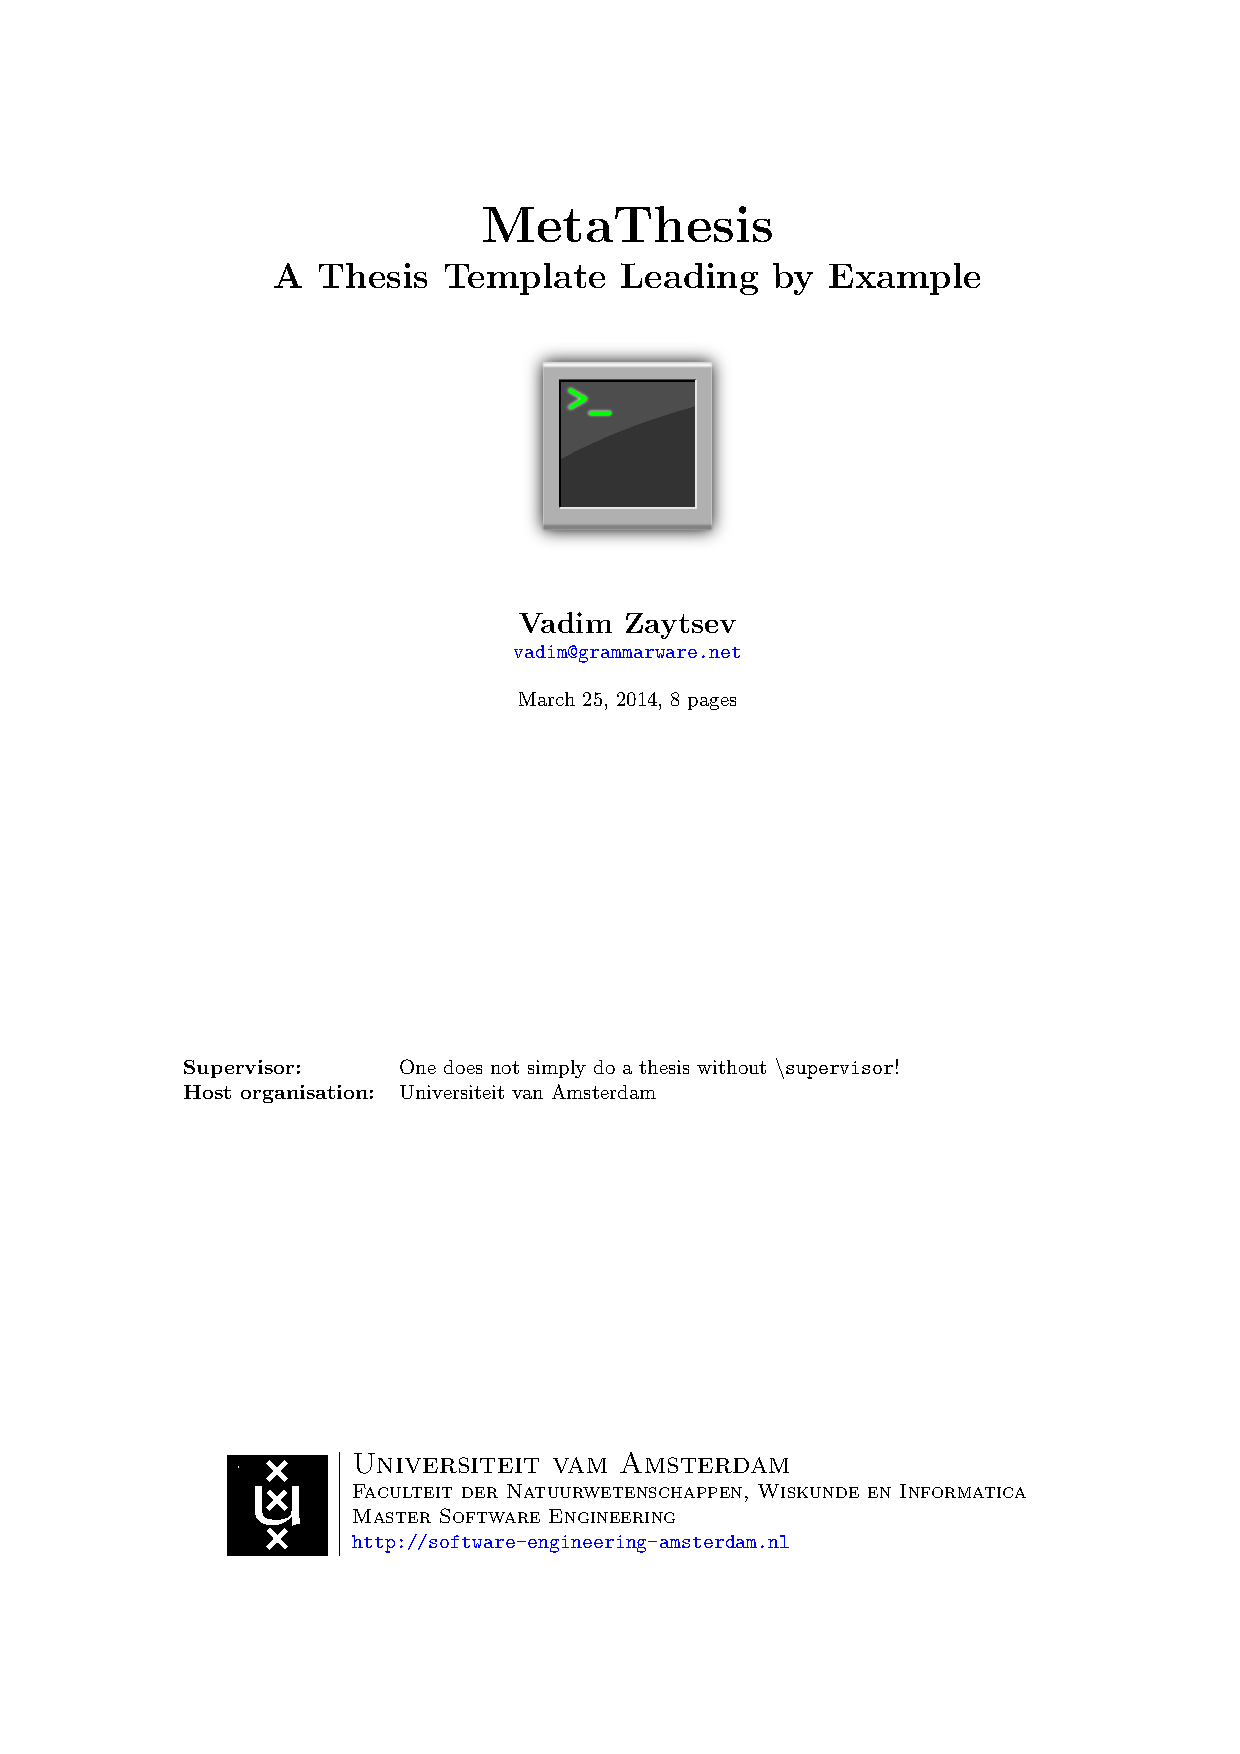
\includegraphics[width=.25\textwidth]{figures/title3.pdf}}
%   \caption{A hypothetical thesis title page without a cover picture (on the left), with an overly large one (in the centre) and with a tiny pic (on the right).}
%   \label{fig:titles}
% \end{figure}

% \section{Abstract}

% A thesis is fine without an abstract, if you do not feel like writing it and
% your supervisor does not feel like enforcing it. If you do want an abstract,
% make it with the \cmd{abstract} command:

% \begin{snippet}
% \begin{verbatim}
% \abstract{This is not a thesis.}
% \end{verbatim}
% \end{snippet}

% The abstract is just like any other section of your thesis, so you can use any
% \LaTeX\ tricks there. If you think that the name ``abstract'' is too abstract
% for your abstract, you can still use \cmd{abstract} without being too
% abstract:

% \begin{snippet}
% \begin{verbatim}
% \abstract[Confession]{I am a cenosillicaphobiac.}
% \end{verbatim}
% \end{snippet}

% Kent Beck~\cite{JohnsonBBCGW93} proposes to have four sentences in a good abstract:

% \begin{enumerate}
%   \item The first states the problem.
%   \item The second states why the problem is a problem.
%   \item The third is the startling sentence.
%   \item The fourth states the implication of the startling sentence.
% \end{enumerate}

% In practice, each of these ``sentences'' can be longer than an actual
% sentence, but it is in general a good rule of thumb to condense the summary of
% your thesis into these four tiny messages. Do not write too much, make it
% tweetable.

% %%%%%%%%%%%%%%%%%%%%%%%%%%%%%%%%%%%%%%%%%%%%%%%%%%%%%%%%%%%%%%%%%%%%%%%%%%%%%%%
% \chapter{Core Chapters}

% The structure of your thesis is up to you and your supervisor. Whatever you
% do, do not consider the guidelines below as dogmas.

% \section{Classic structure}

% \begin{description}
%   \item[Problem statement and motivation.]
%   You describe in detail what problem the research is addressing, and what is
% the motivation to address this problem. There is a concise and objective
% statement of the research questions, hypotheses and goals. It is made clear
% why these questions and goals are important and relevant to the world outside
% the university (assuming it exists). You can already split the main research
% question into subquestions in this chapter. This section also describes an
% analysis of the problem: where does it occur and how, how often, and what are
% the consequences? An important part is also to scope the research: what
% aspects are included and what aspects are deliberately left out, and why?
%   \item[Research method.]
%   Here you describe the methods used to answer the research questions. A good
% structure of this section often follows the subquestions by providing a method
% for each. The research method needs a thorough motivation grounded in theory
% in order to be acceptable. As a part of the method, you can introduce a number
% of hypotheses --- these will be tested by the research, using the methods
% described here. An important part of this section is validation. How will you
% evaluate and validate the outcomes of the research?
%   \item[Background and context.]
%   This chapter contains all the information needed to put the thesis into
% context. It is common to use a revised version of your literature survey for
% this purpose. It is important to explicitly refer from your text to sources
% you have used, they will be listed in your bibliography. For example, you can
% write ``A small number of programming languages account for most language
% use~\cite{MeyerovichR2013}'', where the following entry would be included in
% your bibliography:
% \begin{quote}
% \cite{MeyerovichR2013} Leo A. Meyerovich and Ariel S. Rabkin. Empirical Analysis of Programming Language Adoption. In \emph{Proceedings of the 2013 ACM SIGPLAN International Conference on Object Oriented Programming Systems Languages and Applications}, OOPSLA, pages 1--18. ACM, 2013. \doi{10.1145/2509136.2509515}.
% \end{quote}
% Have a look at \autoref{sec:biblio} to learn more about citation.
%   \item[Research.]
%   This chapter reports on the execution of the research method as described in
% an earlier chapter. If the research has been divided into phases, they are
% introduced, reported on and concluded individually. If needed, this chapter
% could be split up to balance out the sizes of all chapters.
%   \item[Results.]
%   This chapter presents and clarifies the results obtained during the
%   research. The focus should be on the factual results, not the interpretation
%   or discussion. Tables and graphics should be used to increase the clarity of
%   the results where applicable.
%   \item[Analysis and conclusions.]
%   This chapter contains the analysis and interpretation of the results. The
%   research questions are answered as best as possible with the results that
%   were obtained. The analysis also discussed parts of the questions that were
%   left unanswered.

%   An important topic is the validity of the results. What methods of
%   validation were used? Could the results be generalised to other cases? What
%   threats to validity can be identified? There is room here to discuss the
%   results of related scientific literature here as well. How do the results
%   obtained here relate to other work, and what consequences are there? Did
%   your approach work better or worse? Did you learn anything new compared to
%   the already existing body of knowledge? Finally, what could you say in
%   hindsight on the research approach by followed? What could have done better?
%   What lessons have been learned? What could other researchers use from your
%   experience? A separate section should be devoted to ``future work'', i.e.,
%   possible extension points of your work that you have identified. Even other
%   researchers should be able to use those as a starting point.
% \end{description}

% \section{Reporting on replications}

% Here are the guidelines to report on replicated studies~\cite{Carver10}:

% \begin{description}
%   \item[Information about the original study]~\\
%     \begin{description}
%     \item[Research question(s)] that were the basis for the design
%     \item[Participants,] their number and any other relevant characteristics
%     \item[Design] as a graphical or textual description of the experimental design
%     \item[Artefacts,] the description of them and/or links to the artefacts used
%     \item[Context variables] as any important details that affected the design of the study or interpretation of the 
% results
%     \item[Summary of the results] in a brief overview of the major findings
%     \end{description}
%   %
%   \item[Information about the replication]~\\
%     \begin{description}
%     \item[Motivation for conducting the replication] as a 
% description of why the replication was conducted: 
% to validate the results, to broaden the results by 
% changing the participant pool or the artifacts. 
%     \item[Level of interaction with original experimenters.]
% The level of interaction between the original experimenters and the
% replicators should be reported. This interaction could range from none (i.e.
% simply read the  paper) to them being the same people. There is quite a lot of
% discussion of the level of interaction allowed for the replication to be
% ``successful'', but this level should be reported even without  addressing
% the controversy.
%     \item[Changes to the original experiment.] Any changes made to the
% design, participants, artifacts, procedures, data collected and/or analysis
% techniques should be  discussed along with the motivation for the change.
%     \end{description}
%   \item[Comparison of results to original]~\\
%     \begin{description}
%     \item[Consistent results,] when replication results supported 
% results from the original study, and 
%     \item[Differences in results,] when results from the replication 
% did not coincide with the results from the original study. 
% Authors should also discuss how changes made to the 
% experimental design (see above) may have caused 
% these differences. 
%     \end{description}
%     \item[Drawing conclusions across studies]
% \end{description}

% NB: this section contains portions of text repeated directly from Carver~\cite{Carver10} and 
% only slightly massaged. Do not do this for your thesis, write your own thoughts down.

% \section{\LaTeX\ details}

% \subsection{Environments}

% A \LaTeX\ environment is something with opening and closing tags, which look
% like \cmd{begin}\{\texttt{name}\} and \cmd{end}\{\texttt{name}\}. Some useful
% environments to know:

% \begin{center}
% \begin{tabular}{ll}
%   \texttt{itemize}      & bullet lists\\
%   \texttt{enumerate}    & numbered lists\\
%   \texttt{description}  & definition lists\\
%   \hline
%   \texttt{center}       & centered line elements\\
%   \texttt{flushright}   & right aligned lines\\
%   \texttt{flushleft}    & left aligned lines\\
%   \hline
%   \texttt{tabular}      & table\\
%   \texttt{longtable}    & multi-page table (needs the \texttt{longtable} package)\\
%   \texttt{sideways}     & rotates some text\\
%   \texttt{quote}        & block quote\\
%   \texttt{verbatim}     & unformatted text\\
%   \texttt{minipage}     & compound box with elements inside\\
%   \texttt{boxedminipage}& compound box with elements inside and a border around it\\
%   \hline
%   \texttt{table}        & floating table (needs to have \texttt{tabular} nested inside)\\
%   \texttt{figure}       & floating figure\\
%   \texttt{sourcecode}   & floating listing\\
%   \hline
%   \texttt{equation}     & mathematical equation\\
%   \texttt{lstlisting}   & pretty-printed syntax highligted listing\\
%   \texttt{multline}     & mathematical equation spanning over multiple lines\\
%   \texttt{eqnarray}     & system of mathematical equations\\
%   \texttt{gather}       & bundled mathematical equations\\
%   \texttt{align}        & bundled and aligned mathematical equations\\
%   \texttt{array}        & matrix\\
%   \texttt{CD}           & commutative diagrams\\
% \end{tabular}
% \end{center}

% \section{Listings}

% \begin{sourcecode}
% \begin{lstlisting}[language=prolog]
% define(Ps1,G1,G2)
%  :-
%     usedNs(G1,Uses),
%     ps2n(Ps1,N),
%     require(
%       member(N,Uses),
%       'Nonterminal ~q must not be fresh.',
%       [N]),
%     new(Ps1,N,G1,G2),
%     !.
% \end{lstlisting}
% \caption{Code in Prolog}
% \end{sourcecode}

% \begin{sourcecode}
% \begin{lstlisting}[language=sdf]
% module Syntax

% imports Numbers
% imports basic/Whitespace

% exports
%   sorts
%     Program Function Expr Ops Name Newline

%   context-free syntax
%     Function+                          -> Program
%     Name Name+ "=" Expr Newline+       -> Function
%     Expr Ops Expr                      -> Expr      {left,prefer,cons(binary)}
%     Name Expr+                         -> Expr      {avoid,cons(apply)}
%     "if" Expr "then" Expr "else" Expr  -> Expr      {cons(ifThenElse)}
%     "(" Expr ")"                       -> Expr      {bracket}
%     Name                               -> Expr      {cons(argument)}
%     Int                                -> Expr      {cons(literal)}
%     "-"                                -> Ops       {cons(minus)}
%     "+"                                -> Ops       {cons(plus)}
%     "=="                               -> Ops       {cons(equal)}
% \end{lstlisting}
% \caption{Code in SDF}
% \end{sourcecode}

% \begin{sourcecode}
% \begin{lstlisting}[language=Java]
% import types.*;
% import org.antlr.runtime.*;

% public class TestEvaluator 
%     public static void main(String[] args) throws Exception {

%         // Parse file to program
%         ANTLRFileStream input = new ANTLRFileStream(args[0]);
%         FLLexer lexer = new FLLexer(input);
%         CommonTokenStream tokens = new CommonTokenStream(lexer);
%         FLParser parser = new FLParser(tokens);
%         Program program = parser.program();

%         // Parse sample expression
%         input = new ANTLRFileStream(args[1]);
%         lexer = new FLLexer(input);
%         tokens = new CommonTokenStream(lexer);
%         parser = new FLParser(tokens);
%         Expr expr = parser.expr();

%         // Evaluate program
%         Evaluator eval = new Evaluator(program);
%         int expected = Integer.parseInt(args[2]);
% \end{lstlisting}
% \caption{Code in Java}
% \end{sourcecode}

% \begin{sourcecode}
% \begin{lstlisting}[style=mono,language=Python]
% #!/usr/local/bin/python
% # wiki: BGF
% import os
% import sys
% import slpsns
% import elementtree.ElementTree as ET

% # root::nonterminal* production*
% class Grammar:
%   def __init__(self):
%     self.roots = []
%     self.prods = []
%   def parse(self,fname):
%     self.roots = []
%     self.prods = []
%     self.xml = ET.parse(fname)
%     for e in self.xml.findall('root'):
%       self.roots.append(e.text)
%     for e in self.xml.findall(slpsns.bgf_('production')):
%       prod = Production()
%       prod.parse(e)
%       self.prods.append(prod)
% \end{lstlisting}
% \caption{Code in Python}
% \end{sourcecode}

% \chapter{Literature}\label{sec:biblio}

% \textsc{Bib}TeX\ is a JSON-like format for bibliographic entries. Encode each
% source once as a \textsc{Bib}\TeX\ entry, give it a name and refer to it from
% any place in your thesis. The bibliography at the end of the thesis will be
% compiled automatically from those entries that are referenced at least once,
% it will also be automatically sorted and fancyfied (URLs, DOIs, etc).

% DOI is a digital object identifier, it is uniquely and immutably assigned to
% any paper published in a well-established journal or conference proceedings
% and can be used to refer to it. When used in a browser, it resolves to a
% publisher's website where paper can be obtained. Including DOIs in citations
% is considered good practice and lets the readers of your thesis get to the
% text of the paper in one click. Books do not have DOIs, only ISBNs; some
% workshop proceedings and most unofficial publications do not have DOIs. If you
% want to get a DOI assigned to your work such as a piece of code, upload it to
% \href{http://www.figshare.com}{FigShare}.

% Keys in key-value pairs within each \textsc{Bib}\TeX\ entry are never quoted,
% values usually are, but can also be included within curly brackets or left as
% is, which works fine for numbers (e.g., years). If you want to preserve the
% value from any adjustments (e.g., no recapitalisation in titles), use curlies
% \emph{and} quotes. Separate authors and editors by ``and'', which will
% automatically be mapped to commas or left as ``and''s as necessary.

% \section{Books}

% \cite{GruneJacobs} is just as good as the Dragon Book, but newer and has an
% awesome extended bibliography available for free.

% \begin{snippet}
% \begin{verbatim}
% @book{GruneJacobs,
%   author    = "D. Grune and C. J. H. Jacobs",
%   title     = "{Parsing Techniques: A Practical Guide}",
%   series    = "Monographs in Computer Science",
%   edition   = 2,
%   publisher = "Springer",
%   url       = "http://www.cs.vu.nl/~dick/PT2Ed.html",
%   year      = 2008,
% }
% \end{verbatim}
% \end{snippet}

% \section{Journal papers}

% Not all TOSEM papers are hard to read~\cite{GrammarwareAgenda}.

% \begin{snippet}
% \begin{verbatim}
% @article{GrammarwareAgenda,
%   author      = "Paul Klint and Ralf L{\"a}mmel and Chris Verhoef",
%   title       = "{Toward an Engineering Discipline for Grammarware}",
%   journal     = "ACM Transactions on Software Engineering Methodology (TOSEM)",
%   volume      = 14,
%   number      = 3,
%   year        = 2005,
%   pages       = "331--380",
% }
% \end{verbatim}
% \end{snippet}

% \section{Conference papers}

% There is no limit to how many grammars can be used in one paper, but the
% current record stands at 569~\cite{Micropatterns2013}.

% \begin{snippet}
% \begin{verbatim}
% @inproceedings{Micropatterns2013,
%   author = "Vadim Zaytsev",
%   title = "{Micropatterns in Grammars}",
%   booktitle = "{Proceedings of the Sixth International Conference on Software Language Engineering
%                 (SLE 2013)}",
%   year = 2013,
%   editor = "Martin Erwig and Richard F. Paige and Eric Van Wyk",
%   volume = "8225",
%   series = "LNCS",
%   pages = "117--136",
%   address = "Switzerland",
%   month = oct,
%   publisher = "Springer International Publishing",
%   doi = "10.1007/978-3-319-02654-1_7",
% }
% \end{verbatim}
% \end{snippet}

% \section{Theses}

% The seventh PhD student of Paul Klint was Jan Rekers~\cite{Rekers92}.

% \begin{snippet}
% \begin{verbatim}
% @phdthesis{Rekers92,
%  author   = "J. Rekers",
%  title    = "{Parser Generation for Interactive Environments}",
%  school   = "University of Amsterdam",
%  year     = 1992,
%  url      = "http://homepages.cwi.nl/~paulk/dissertations/Rekers.pdf",
% }
% \end{verbatim}
% \end{snippet}

% There is also \texttt{mastersthesis} type with exactly the same structure for
% referring to Master's theses.

% \section{Technical reports}

% The original seminal work introducing two-level grammars was never published
% in any book or conference, but there is a technical report explaining
% it~\cite{Wijngaarden65}. SMC, or \emph{Stichting Matematisch Centrum}, was the
% old name of CWI fifty years ago.

% \begin{snippet}
% \begin{verbatim}
% @techreport{Wijngaarden65,
%         author      = "Adriaan van Wijngaarden",
%         title       = "{Orthogonal Design and Description of a Formal Language}",
%         month       = oct,
%         year        = 1965,
%         institution = "SMC",
%         type        = "{MR 76}",
%         url         = "http://www.fh-jena.de/~kleine/history/languages/VanWijngaarden-MR76.pdf",
% }
% \end{verbatim}
% \end{snippet}

% \section{Wikipedia}

% You do not refer to Wikipedia from academic writing, it works the other way around.

% \section{Anything else}

% You can refer to pretty much anything (websites, blog posts, software) through
% \texttt{misc} type of entry~\cite{ANTLR}:

% \begin{snippet}
% \begin{verbatim}
% @misc{ANTLR,
%  author       = "Terence Parr",
%  title        = "{ANTLR---ANother Tool for Language Recognition}",
%  howpublished = "Software",
%  url          = "http://antlr.org",
%  year         = "2008"
% }
% \end{verbatim}
% \end{snippet}

{%\tiny
\bibliographystyle{ieeetr}
\bibliography{thesis}
}

\end{document}
